% =====================================================================
%  第 2 章 路径积分形式 —— ch02b（§2.6–§2.7）
%  页段：PDF 109–138（原书 p.108–137）
% =====================================================================

% [原文 p.108]
渐近展开
\[
I(\lambda)\simeq n_-\int_{C^-_\lambda}+n_+\int_{C^+_\lambda}
\]
会呈现跳跃
\[
\begin{cases}
n_+\mapsto n_+,\\
n_-\mapsto n_-\pm n_+.
\end{cases}
\]
这是可行的，因为它不改变 $I(\lambda)$ 的首阶渐近行为；该行为由占主导的项 $n_+\int_{C^+_\lambda}$ 给出。

\takeaway{§2.5 系统整理复积分 $\int e^{\lambda f}g$ 在 $\lambda\to\infty$ 时的渐近方法：拉普拉斯方法把主导贡献归到实轴上 $f$ 的最大点，最速下降法把积分围道变形到鞍点处 $\operatorname{Im}f$ 为常数的下降曲线上，莫尔斯流刻画出这些曲线并给出围绕鞍点的局部模型；当围道在变形中扫过斯托克斯线时，鞍点的相对权重会按斯托克斯现象跳变，这正是后面连接公式的来源。}

\section{半经典近似}

本节的目标是用最速下降法，计算费曼核
\[
K(x'',t'';x',t')=\int_{x(t')=x'}^{x(t'')=x''}[\mathcal{D}x(t)]\,
\ee^{\frac{\ii}{\hs}S[x(t)]}
\]
在经典极限 $\hs\to0$ 下的渐近首阶贡献。为简单起见，我们聚焦于一维情形。

\subsection{半经典的费曼核}

$S$ 的鞍点是经典轨迹 $x_{cl}(t)$。我们把一般路径 $x(t)$ 写成
\[
x(t)=x_{cl}(t)+\gamma(t),
\]
其中 $\gamma(t)$ 满足端点条件
\[
\gamma(t')=\gamma(t'')=0.
\]
把 $S[x(t)]$ 在经典轨迹 $x_{cl}(t)$ 附近展开，得到
\[
\begin{aligned}
S[x(t)]&=\int_{t'}^{t''}\left(\frac{m}{2}\dot x^2-V(x)\right)\rd t\\
&=S[x_{cl}(t)]+\int_{t'}^{t''}\left(\frac{m}{2}\dot\gamma^2-\frac12V''(x_{cl})\gamma^2\right)\rd t+O(\gamma^3).
\end{aligned}
\]
于是最速下降法给出如下渐近首阶贡献：
\[
K(x'',t'';x',t')\simeq \ee^{\frac{\ii}{\hs}S[x_{cl}(t)]}
\int_{\gamma(t')=0}^{\gamma(t'')=0}[\mathcal{D}\gamma(t)]\,
\ee^{\frac{\ii}{\hs}\int_{t'}^{t''}\left(\frac{m}{2}\dot\gamma^2-\frac12V''(x_{cl})\gamma^2\right)\rd t}
\qquad\text{当 }\hs\to0.
\]
这就是所谓的半经典近似。

记半经典费曼核为
\[
K_{sc}(x'',t'';x',t'):=\ee^{\frac{\ii}{\hs}S[x_{cl}(t)]}
\int_{\gamma(t')=0}^{\gamma(t'')=0}[\mathcal{D}\gamma(t)]\,
\ee^{\frac{\ii}{\hs}\int_{t'}^{t''}\left(\frac{m}{2}\dot\gamma^2-\frac12V''(x_{cl})\gamma^2\right)\rd t}.
\]
应用关于高斯路径积分的结果，半经典费曼核成为
\[
K_{sc}(x'',t'';x',t')=
\left(\frac{m}{\pi\ii\hs\det A}\right)^{\frac12}\ee^{\frac{\ii}{\hs}S[x_{cl}(t)]},
\]
其中 $A$ 是椭圆算子
\[
A=-\frac{\rd^2}{\rd t^2}-\frac1m V''(x_{cl}(t)).
\]

% [原文 p.109]
本小节的主要目标是证明如下半经典公式
\[
K_{sc}(x'',t'';x',t')=
\left(\frac{m}{2\pi\ii\hs\varphi_0(t'')}\right)^{\frac12}
\ee^{\frac{\ii}{\hs}S[x_{cl}(t)]},
\]
其中 $\varphi_0(t)$ 是初值问题
\[
\begin{cases}
\left(-\dfrac{\rd^2}{\rd t^2}-\dfrac1m V''(x_{cl}(t))\right)\varphi_0(t)=0,\\[2mm]
\varphi_0(t')=0,\qquad \varphi_0'(t')=1
\end{cases}
\]
的解。

\subsubsection*{行列式计算}

记
\[
\Theta(t)=\frac1m V''(x_{cl}(t)).
\]
我们给出
\[
\det A=\det\left(-\frac{\rd^2}{\rd t^2}-\Theta(t)\right)
\]
的一个直观计算，它来自 Coleman [10]。

思路是分析带 $t=t'$ 处初值条件的本征值问题
\[
\begin{cases}
A\varphi_\lambda(t)=\lambda\varphi_\lambda(t),\\
\varphi_\lambda(t')=0,\qquad \varphi'_\lambda(t')=1.
\end{cases}
\]
对任意 $\lambda$，上述初值问题都有唯一解 $\varphi_\lambda(t)$。关键在于观察到
\[
\varphi_\lambda(t'')=0
\]
当且仅当 $\lambda$ 是 $A$ 在相应狄利克雷（Dirichlet）边值问题
\[
\begin{cases}
A\varphi_\lambda(t)=\lambda\varphi_\lambda(t),\\
\varphi_\lambda(t')=\varphi_\lambda(t'')=0
\end{cases}
\]
下的本征值。

现在考虑另一个算子
\[
\tilde A=-\frac{\rd^2}{\rd t^2}-\tilde\Theta(t),
\]
同样对
\[
\begin{cases}
\tilde A\tilde\varphi_\lambda(t)=\lambda\tilde\varphi_\lambda(t),\\
\tilde\varphi_\lambda(t')=0,\qquad \tilde\varphi'_\lambda(t')=1
\end{cases}
\]
解出 $\tilde\varphi_\lambda(t)$。

% [原文 p.110]
于是我们断言
\[
\frac{\det(A-\lambda)}{\det(\tilde A-\lambda)}=
\frac{\varphi_\lambda(t'')}{\tilde\varphi_\lambda(t'')}.
\tag{$*$}
\]
直观上，这可以通过“观察”得到：两端都是 $\lambda$ 的亚纯函数，零点在 $A$ 的本征值处，极点在 $\tilde A$ 的本征值处（细致的分析表明，这些零点与极点都是单重的）。令
\[
f(\lambda)=\frac{\det(A-\lambda)}{\det(\tilde A-\lambda)},
\qquad
g(\lambda)=\frac{\varphi_\lambda(t'')}{\tilde\varphi_\lambda(t'')}.
\]
那么上述考虑说明 $\dfrac{f(\lambda)}{g(\lambda)}$ 是 $\C$ 上的整函数。

接下来分析 $f(\lambda)$ 与 $g(\lambda)$ 当 $\lambda\to\infty$ 时的行为。首先，
\[
\lim_{\substack{\lambda\to\infty\\ \lambda\notin\R_+}}f(\lambda)=1.
\]
定性上可以这样理解。对狄利克雷边值问题，算子 $-\dfrac{\rd^2}{\rd t^2}$ 有本征向量
\[
u_n(t)=\sin\left(\frac{n\pi}{t''-t'}(t-t')\right),
\]
本征值为 $\left(\dfrac{n\pi}{t''-t'}\right)^2$。因此平移后的算子 $-\dfrac{\rd^2}{\rd t^2}-\lambda$ 的本征值为
\[
\mu_n=\left(\frac{n\pi}{t''-t'}\right)^2-\lambda.
\]
在 $\lambda\to\infty$、$\lambda\notin\R_+$ 的极限下，全部本征值满足 $\abs{\mu_n}\to+\infty$。因此在 $\lambda\to\infty$、$\lambda\notin\R_+$ 时，$\Theta(t)$ 相比算子 $-\dfrac{\rd^2}{\rd t^2}-\lambda$ 非常小。这一小扰动在该极限下影响可以忽略。于是自然地期待
\[
\lim_{\substack{\lambda\to\infty\\ \lambda\notin\R_+}}f(\lambda)=1.
\]
其次，考虑极限
\[
\lim_{\substack{\lambda\to\infty\\ \lambda\notin\R_+}}g(\lambda).
\]
为分析该极限，先考虑非齐次问题
\[
\begin{cases}
\left(-\dfrac{\rd^2}{\rd t^2}-\lambda\right)u=f,\\[2mm]
u(t')=0,\qquad u'(t')=0.
\end{cases}
\]
它由
\[
u(t)=-\int_{t'}^{t}\frac{1}{\sqrt\lambda}\sin\left(\sqrt\lambda(t-s)\right)f(s)\,\rd s
\]
唯一解出。相应的格林算子为
\[
G(f)(t):=-\int_{t'}^{t}\frac{1}{\sqrt\lambda}\sin\left(\sqrt\lambda(t-s)\right)f(s)\,\rd s.
\]

% [原文 p.111]
考虑原来的边值问题
\[
\begin{cases}
\left(-\dfrac{\rd^2}{\rd t^2}-\lambda-\Theta(t)\right)\varphi_\lambda(t)=0,\\[2mm]
\varphi_\lambda(t')=0,\qquad \varphi'_\lambda(t')=1.
\end{cases}
\]
我们把 $\varphi_\lambda(t)$ 写成
\[
\varphi_\lambda(t)=\varphi^{(0)}_\lambda(t)+u(t),
\]
其中 $\varphi^{(0)}_\lambda(t)$ 求解
\[
\begin{cases}
\left(-\dfrac{\rd^2}{\rd t^2}-\lambda\right)\varphi^{(0)}_\lambda=0,\\[2mm]
\varphi^{(0)}_\lambda(t')=0,\qquad \varphi^{(0)'}_\lambda(t')=1.
\end{cases}
\]
这样的 $\varphi^{(0)}_\lambda$ 可显式求出：
\[
\varphi^{(0)}_\lambda(t)=\frac{1}{\sqrt\lambda}\sin\left(\sqrt\lambda(t-t')\right).
\]
于是 $\varphi_\lambda(t)$ 满足的方程变为
\[
\begin{cases}
\left(-\dfrac{\rd^2}{\rd t^2}-\lambda\right)u(t)=\Theta(t)\left(\varphi^{(0)}_\lambda(t)+u(t)\right),\\[2mm]
u(t')=0,\qquad u'(t')=0.
\end{cases}
\]
利用上面的格林算子，这等价于
\[
u=G\left(\Theta\left(\varphi^{(0)}_\lambda+u\right)\right).
\]
把它改写为
\[
(1-G\circ\hat\Theta)u=G\circ\hat\Theta\left(\varphi^{(0)}_\lambda\right),
\]
其中 $\hat\Theta$ 是算子
\[
\hat\Theta(u)(t)=\Theta(t)u(t).
\]
于是得到扰动解
\[
u=(1-G\circ\hat\Theta)^{-1}G\circ\hat\Theta\left(\varphi^{(0)}_\lambda\right)
=\sum_{n=1}^{\infty}(G\circ\hat\Theta)^n\left(\varphi^{(0)}_\lambda\right).
\]
由这一表达式可知，修正项 $u$ 具有渐近行为
\[
u=O\left(\frac{\Theta}{\sqrt\lambda}\right)\varphi^{(0)}_\lambda,
\]
它在 $\lambda\to\infty$、$\lambda\notin\R_+$ 的极限下比 $\varphi^{(0)}_\lambda$ 小。由此可知
\[
\lim_{\substack{\lambda\to\infty\\ \lambda\notin\R_+}}g(\lambda)
=\lim_{\substack{\lambda\to\infty\\ \lambda\notin\R_+}}
\frac{\varphi^{(0)}_\lambda(t'')}{\tilde\varphi^{(0)}_\lambda(t'')}=1.
\]

% [原文 p.112]
结合上面两个结果，得到
\[
\lim_{\substack{\lambda\to\infty\\ \lambda\notin\R_+}}
\frac{f(\lambda)}{g(\lambda)}=1.
\]
由于 $f(\lambda)/g(\lambda)$ 是整函数，由此可知 $f(\lambda)/g(\lambda)=1$。这就证明了 $(*)$。

把 $(*)$ 改写为
\[
\frac{\det(A-\lambda)}{\varphi_\lambda(t'')}=
\frac{\det(\tilde A-\lambda)}{\tilde\varphi_\lambda(t'')}.
\]
由此可知
\[
\det A=c\varphi_0(t''),
\]
其中 $c$ 是不依赖势 $V$ 的常数。常数 $c$ 可由自由情形的结果确定，该情形下 $\tilde A=-\dfrac{\rd^2}{\rd t^2}$。在自由情形，由 §2.3.2 知道
\[
\det(\tilde A)=\det\left(-\frac{\rd^2}{\rd t^2}\right)=2(t''-t').
\]
另一方面，微分方程
\[
\begin{cases}
-\dfrac{\rd^2}{\rd t^2}\tilde\varphi_0(t)=0,\\[2mm]
\tilde\varphi_0(t')=0,\qquad \tilde\varphi'_0(t')=1
\end{cases}
\]
的解为
\[
\tilde\varphi_0(t)=t-t'.
\]
于是
\[
c=\frac{\det\tilde A}{\tilde\varphi_0(t'')}=2.
\]
因此
\[
\det A=2\varphi_0(t'').
\]
我们得到了所承诺的半经典费曼核公式
\[
K_{sc}(x'',t'';x',t')=
\left(\frac{m}{2\pi\ii\hs\varphi_0(t'')}\right)^{\frac12}
\ee^{\frac{\ii}{\hs}S[x_{cl}(t)]},
\]
其中 $\varphi_0(t)$ 是初值问题
\[
\begin{cases}
\left(-\dfrac{\rd^2}{\rd t^2}-\dfrac1m V''(x_{cl}(t))\right)\varphi_0(t)=0,\\[2mm]
\varphi_0(t')=0,\qquad \varphi_0'(t')=1
\end{cases}
\]
的解。

\subsection{雅可比场}

半经典费曼核中出现的函数 $\varphi_0(t)$，在几何上可以用雅可比场来解释。我们说明这一联系，并给出几个应用。

% [原文 p.113]
考虑所有在初始时刻 $t=t'$ 从 $x'$ 出发的经典轨迹。它们由 $t=t'$ 处的初速度 $v'$ 参数化。记 $x_{cl}(t;v')$ 为满足运动方程初值问题
\[
\begin{cases}
m\ddot x_{cl}+V'(x_{cl})=0,\\
x_{cl}(t';v')=0,\qquad \dot x_{cl}(t';v')=v'
\end{cases}
\]
的经典轨迹。这里 $\dot{(\ )}$ 表示 $\dfrac{\pa(\ )}{\pa t}$。于是 $x_{cl}(t;v')$ 给出了一族由 $v'$ 参数化的经典轨迹。

考虑这族轨迹关于参数 $v'$ 的变分
\[
J(t;v')=\frac{\pa}{\pa v'}x_{cl}(t;v').
\]
它称为\emph{雅可比场}（Jacobi field）。把运动方程 $m\ddot x_{cl}+V'(x_{cl})=0$ 关于 $v'$ 求导，可知雅可比场满足
\[
m\frac{\pa^2}{\pa t^2}J+V''(x_{cl})J=0,
\]
该方程称为\emph{雅可比方程}（Jacobi equation）。

\begin{center}
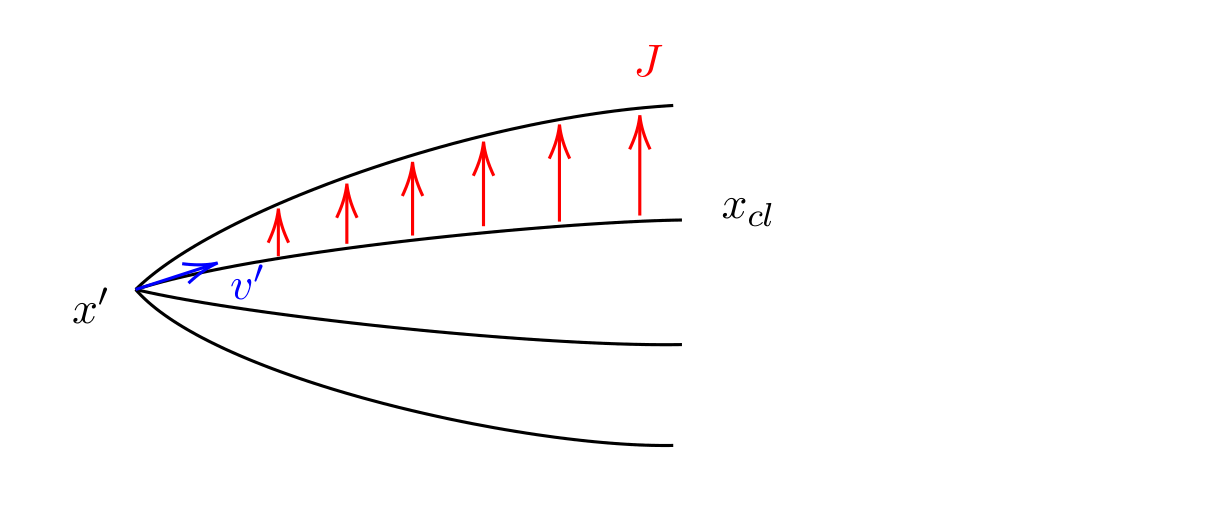
\includegraphics[width=0.55\textwidth]{figures/fig_p114_a.png}
\end{center}
% [图：原书 p.113，图内文字照原样保留]

初值条件给出
\[
\begin{cases}
x_{cl}(t';v')=0,\\
\dot x_{cl}(t';v')=v'
\end{cases}
\quad\Longrightarrow\quad
\begin{cases}
J(t';v')=0,\\
\dot J(t';v')=1.
\end{cases}
\]
因此 $J(t;v')$ 满足如下初值问题
\[
\begin{cases}
\left(-\dfrac{\pa^2}{\pa t^2}-\dfrac1m V''(x_{cl})\right)J=0,\\[2mm]
J|_{t=t'}=0,\qquad \dot J|_{t=t'}=1.
\end{cases}
\]
于是 §2.6.1 中行列式里的函数 $\varphi_0(t)$，正是雅可比场
\[
\varphi_0=J.
\]

\begin{remark}{2.6.1}
  使 $J(t'';v')=0$ 的点 $t''$ 称为\emph{共轭点}（conjugate point）。出现共轭点，意味着有一族经典轨迹从 $t=t'$ 的同一个点出发，并且在 $t=t''$ 终止于同一个点。
\end{remark}

% [原文 p.114]
\begin{center}
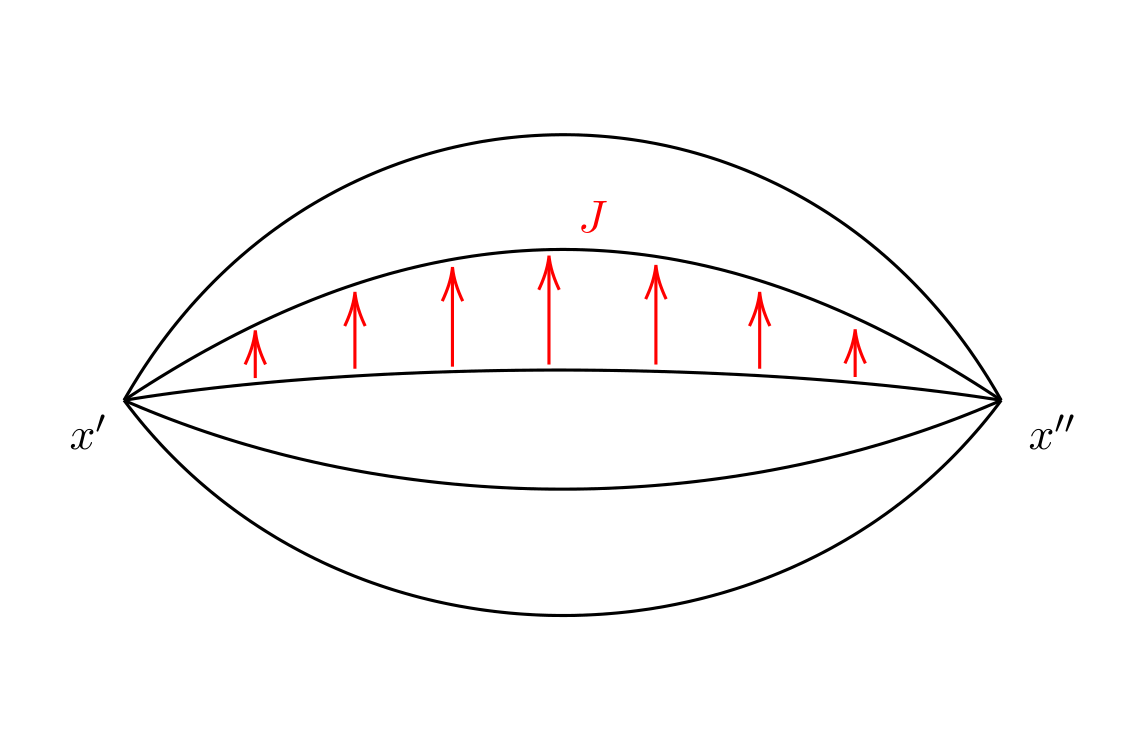
\includegraphics[width=0.7\textwidth]{figures/fig_p115_a.png}
\end{center}
% [图：原书 p.114，图内文字照原样保留]

记
\[
S_{cl}(x'',t'';x',t'):=\int_{t'}^{t''}
\left(\frac{m}{2}\dot x_{cl}^2-V(x_{cl})\right)\rd t
\]
为从 $x(t')=x'$ 出发、终止于 $x(t'')=x''$ 的经典轨迹 $x(t)$ 上的作用量。由经典力学知道，$S_{cl}(x'',t'';x',t')$ 满足\emph{哈密顿–雅可比方程}
\[
\begin{cases}
\dfrac{\pa S_{cl}}{\pa x''}=p(t''),\qquad
\dfrac{\pa S_{cl}}{\pa x'}=-p(t')=-mv',\\[3mm]
\dfrac{\pa S_{cl}}{\pa t''}=-E,\qquad
\dfrac{\pa S_{cl}}{\pa t'}=E.
\end{cases}
\]
这里 $p(t)=m\dot x_{cl}(t)$ 是 $t$ 时刻的共轭动量，$E=\frac12 m\dot x_{cl}^2+V(x_{cl})$ 是沿轨迹 $x_{cl}$ 的能量。由此可知
\[
\frac{\pa^2 S_{cl}}{\pa x'\pa x''}
=-\frac{\pa p(t')}{\pa x''}=-m\frac{\pa v'}{\pa x''}=-\frac{m}{J(t'')}
\quad\Longrightarrow\quad
\frac{1}{J(t'')}=-\frac1m\frac{\pa^2 S_{cl}}{\pa x'\pa x''}.
\]
于是经典路径 $x_{cl}(t)$ 的半经典贡献也可写成
\[
\left(\frac{m}{2\pi\ii\hs\varphi_0(t'')}\right)^{\frac12}
\ee^{\frac{\ii}{\hs}S_{cl}}
=\left(\frac{m}{2\pi\ii\hs J(t'')}\right)^{\frac12}
\ee^{\frac{\ii}{\hs}S_{cl}}
=\left(\frac{\ii}{2\pi\hs}\frac{\pa^2 S_{cl}}{\pa x'\pa x''}\right)^{\frac12}
\ee^{\frac{\ii}{\hs}S_{cl}}.
\]
一般地，如果有若干条经典轨迹在 $t=t'$ 从 $x'$ 出发、在 $t=t''$ 到达 $x''$，那么半经典费曼核就是所有经典轨迹贡献之和
\[
K_{sc}(x'',t'';x',t')
=\sum_{\substack{x_{cl}\\ x_{cl}(t')=x'\\ x_{cl}(t'')=x''}}
\left(\frac{\ii}{2\pi\hs}\frac{\pa^2 S_{cl}}{\pa x'\pa x''}\right)^{\frac12}
\ee^{\frac{\ii}{\hs}S_{cl}},
\]
其中 $S_{cl}(x'',t'';x',t')=S[x_{cl}(t)]$ 是对应经典轨迹上经典作用量的值。这称为\emph{范弗莱克–泡利–莫雷特公式}（Van Vleck–Pauli–Morette formula）。

\begin{example}{2.6.2（自由粒子）}
  经典轨迹是一条直线。给定初始点 $(x',t')$ 与终点 $(x'',t'')$，唯一的经典轨迹是
  \[
  x_{cl}(t)=\frac{x'(t''-t)}{t''-t'}+\frac{x''(t-t')}{t''-t'}.
  \]
  于是
  \[
  S_{cl}(x'',t'';x',t')=\int_{t'}^{t''}\frac12 m\dot x_{cl}(t)^2\,\rd t
  =\frac{m}{2}\frac{(x''-x')^2}{t''-t'},
  \]
  由此
  \[
  \Longrightarrow\quad
  \frac{\pa^2 S_{cl}}{\pa x'\pa x''}=-\frac{m}{t''-t'},
  \]
  \[
  \Longrightarrow\quad
  K_{sc}(x'',t'';x',t')=
  \left(\frac{m}{2\pi\ii\hs(t''-t')}\right)^{\frac12}
  \ee^{\frac{\ii}{\hs}\frac{m(x''-x')^2}{2(t''-t')}}.
  \]
  在自由情形，半经典近似是精确的，即 $K_{sc}=K$。
\end{example}

% [原文 p.115]
\begin{example}{2.6.3（谐振子）}
  考虑简谐振子
  \[
  S[x(t)]=\int_{t'}^{t''}\left(\frac{m}{2}\dot x^2-\frac{m}{2}\omega^2x^2\right)\rd t.
  \]
  经典轨迹的运动方程为
  \[
  \ddot x+\omega^2x=0.
  \]
  当 $\omega(t''-t')\notin\Z\pi$ 时，从 $t=t'$ 的 $x'$ 到 $t=t''$ 的 $x''$ 存在唯一的经典轨迹
  \[
  x_{cl}(t)=\frac{\sin\omega(t''-t)}{\sin\omega(t''-t')}x'
  +\frac{\sin\omega(t-t')}{\sin\omega(t''-t')}x''.
  \]
  令
  \[
  T:=t''-t'.
  \]
  则
  \[
  \begin{aligned}
  S_{cl}(x'',t'';x',t')
  &=\int_{t'}^{t''}\left(\frac{m}{2}\dot x_{cl}^2-\frac{m}{2}\omega^2x_{cl}^2\right)\rd t\\
  &=\frac{m\omega}{2\sin\omega T}\left[((x')^2+(x'')^2)\cos\omega T-2x'x''\right].
  \end{aligned}
  \]
  \[
  \Longrightarrow\quad
  \frac{\pa^2 S_{cl}}{\pa x'\pa x''}=-\frac{m\omega}{\sin\omega T},
  \]
  \[
  \Longrightarrow\quad
  K_{sc}(x'',t'';x',t')=
  \left(\frac{\ii}{2\pi\hs}\frac{\pa^2 S_{cl}}{\pa x'\pa x''}\right)^{\frac12}
  \ee^{\frac{\ii}{\hs}S_{cl}}
  =\left(\frac{m\omega}{2\pi\ii\hs\sin\omega T}\right)^{\frac12}
  \ee^{\frac{\ii}{\hs}S_{cl}}.
  \]
  对谐振子，半经典近似同样是精确的：$K_{sc}=K$。
\end{example}

\subsection{时间切片方法}

经典路径 $x_{cl}(t)$ 对费曼核的半经典贡献
\[
\ee^{\frac{\ii}{\hs}S[x_{cl}(t)]}
\int_{\gamma(t')=0}^{\gamma(t'')=0}[\mathcal{D}\gamma(t)]\,
\ee^{\frac{\ii}{\hs}\int_{t'}^{t''}\left(\frac{m}{2}\dot\gamma^2
-\frac12V''(x_{cl})\gamma^2\right)\rd t}
=\left(\frac{m}{\pi\ii\hs\det A}\right)^{\frac12}
\ee^{\frac{\ii}{\hs}S[x_{cl}(t)]},
\]
其中
\[
A=-\frac{\rd^2}{\rd t^2}-\frac1m V''(x_{cl}(t)),
\]
也可以从对路径作时间切片、再取极限的启发式计算来理解。

% [原文 p.116]
\begin{center}
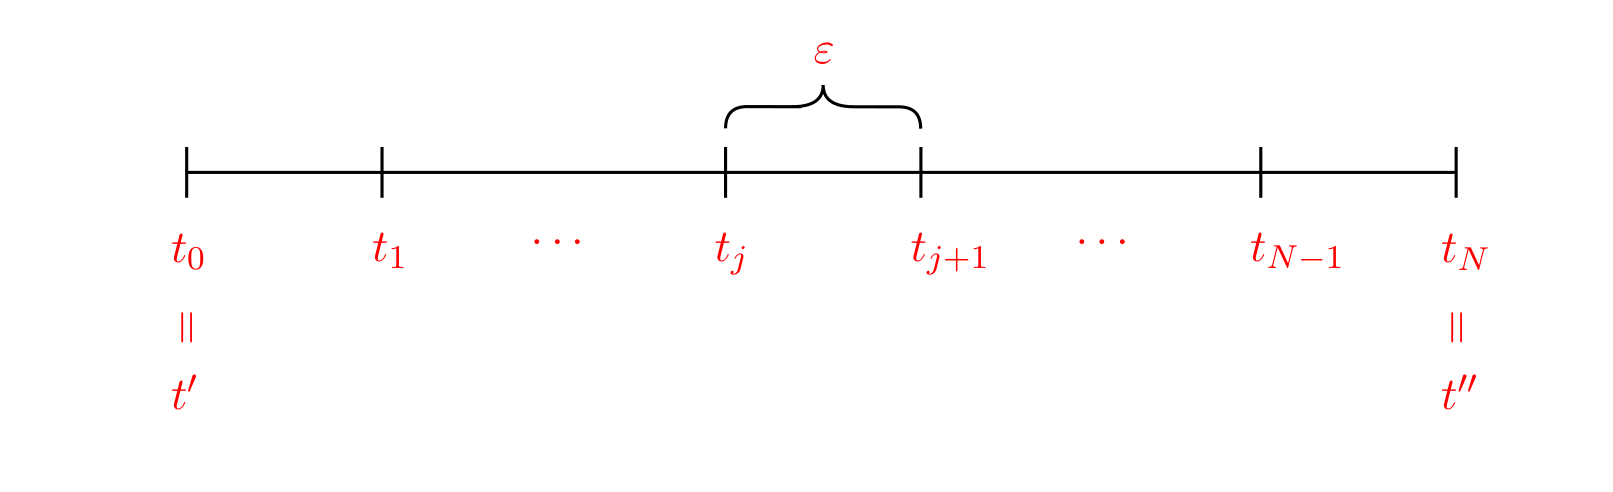
\includegraphics[width=0.7\textwidth]{figures/fig_p117_a.png}
\end{center}
% [图：原书 p.116，图内文字照原样保留]

我们把时间区间 $[t',t'']$ 分成 $N$ 个宽度为 $\eps=\dfrac{t''-t'}{N}$ 的小区间。令
\[
\omega_j^2:=\frac{V''(x_{cl}(t_j))}{m}
\]
表示 $V''(x_{cl})$ 在离散点 $t=t_j$ 处的值。按构造，
\[
\begin{aligned}
&\int_{\gamma(t')=0}^{\gamma(t'')=0}[\mathcal{D}\gamma(t)]\,
\ee^{\frac{\ii}{\hs}\int_{t'}^{t''}\left(\frac{m}{2}\dot\gamma^2
-\frac12V''(x_{cl})\gamma^2\right)\rd t}\\
&=\lim_{\eps\to0}\left(\frac{m}{2\pi\ii\hs\eps}\right)^{\frac N2}
\int\prod_{j=1}^{N-1}\rd x_j\,
\ee^{\frac{\ii}{\hs}\sum\limits_{j=0}^{N-1}
\left[\frac{m}{2}\left(\frac{x_{j+1}-x_j}{\eps}\right)^2
-\frac{m\omega_j^2}{2}x_j^2\right]\eps}
\quad\text{这里 }x_0:=0,\ x_N:=0\\
&=\lim_{\eps\to0}\left(\frac{m}{2\pi\ii\hs\eps}\right)^{\frac N2}
\int\prod_{j=1}^{N-1}\rd x_j\,
\ee^{\frac{\ii m}{2\hs\eps}\mathbf{x}^tA_N\mathbf{x}}
\qquad\text{这里 }\mathbf{x}=(x_1,\dots,x_{N-1})\\
&=\lim_{\eps\to0}\left(\frac{m}{2\pi\ii\hs\eps\det A_N}\right)^{\frac12}.
\end{aligned}
\]
这里 $A_N$ 是 $(N-1)\times(N-1)$ 矩阵
\[
A_N=\begin{pmatrix}
2-\eps^2\omega_1^2 & -1 & & & 0\\
-1 & 2-\eps^2\omega_2^2 & \ddots & & \\
& \ddots & \ddots & \ddots & \\
& & \ddots & 2-\eps^2\omega_{N-2}^2 & -1\\
0 & & & -1 & 2-\eps^2\omega_{N-1}^2
\end{pmatrix}.
\]
令 $u_0=\eps$，并对 $1\le j\le N-1$ 定义
\[
u_j=\eps\det
\begin{pmatrix}
2-\eps^2\omega_1^2 & -1 & & & 0\\
-1 & 2-\eps^2\omega_2^2 & \ddots & & \\
& \ddots & \ddots & \ddots & \\
& & \ddots & 2-\eps^2\omega_{j-1}^2 & -1\\
0 & & & -1 & 2-\eps^2\omega_j^2
\end{pmatrix}.
\]
于是有递推关系
\[
\frac{u_{j+1}-2u_j+u_{j-1}}{\eps^2}+\omega_{j+1}^2u_j=0,
\qquad 1\le j\le N-2.
\]
在连续极限 $\eps\to0$ 下，它成为 $u(t)$（$u_j=u(t_j)$）的微分方程
\[
\ddot u(t)+\omega^2(t)u(t)=0.
\]

% [原文 p.117]
这里 $\omega^2(t)=V''(x_{cl}(t))/m$。初值条件
\[
u_0=\eps,\qquad \frac{u_1-u_0}{\eps}=1-\eps^2\omega_1^2
\]
化为初值条件
\[
u(t')=0,\qquad u'(t')=1.
\]
由此可知
\[
\lim_{\eps\to0}\eps\det A_N=u(t''),
\]
其中 $u(t)$ 满足
\[
\begin{cases}
\ddot u(t)+\dfrac1m V''(x_{cl}(t))u(t)=0,\\[2mm]
u(t')=0,\qquad u'(t')=1.
\end{cases}
\]
这与我们先前得到的结果相同。

\takeaway{本节把驻定相位近似用于路径积分，得到半经典费曼核：领头贡献来自经典轨道，二阶变分由雅可比场决定；由此导出范弗莱克–泡利–莫雷特公式，并用时间切片方法独立验证了行列式的连续极限。}

\section{格林函数}

\subsection{固定能量下的格林函数}

研究薛定谔方程时，转到能量本征态、研究固定能量的定态解很有用。在路径积分表述中，我们因此通过\emph{推迟费曼核}（retarded Feynman kernel）$\theta(t)K(x'',t;x',0)$ 的傅里叶变换，来定义固定能量下的格林函数 $G$。这里
\[
\theta(t)=\begin{cases}1,& t\ge0,\\ 0,& t<0\end{cases}
\]
是赫维赛德（Heaviside）阶跃函数。具体地说，
\[
\begin{aligned}
G(x'',x';E)
&:=\frac1{\ii\hs}\int_{-\infty}^{+\infty}\rd T\,
\ee^{\ii(E+\ii\eps)T/\hs}\theta(T)K(x'',T;x',0)\\
&=\frac1{\ii\hs}\int_0^{+\infty}\rd T\,
\ee^{\ii(E+\ii\eps)T/\hs}K(x'',T;x',0)\\
&=\frac1{\ii\hs}\int_0^{+\infty}\rd T\,
\ee^{\ii(E+\ii\eps)T/\hs}\mel{x''}{\ee^{-\ii\wh HT/\hs}}{x'}\\
&=\mel{x''}{\frac1{E-\wh H+\ii\eps}}{x'}.
\end{aligned}
\]
这里按照分布论中的惯例，引入小正数 $\eps>0$ 以保证积分收敛，最终取 $\eps\to0^+$。

格林函数 $G(x'',x';E)$ 在区域 $\Imag E>0$ 内解析，这反映了傅里叶变换下的推迟性。知道格林函数之后，可以通过傅里叶逆变换还原费曼核
\[
K(x'',T;x',0)=\frac{\ii}{2\pi}\int_{\R}\rd E\,
\ee^{-\ii ET/\hs}G(x'',x';E).
\]

% [原文 p.118]
\begin{remark}{2.7.1}
  作为 $\eps\to0^+$ 方法的一个例证，常用如下分布恒等式
  \[
  \lim_{\eps\to0^+}\frac1{x\pm\ii\eps}
  =\mp\ii\pi\delta(x)+\mathrm{P.V.}\left(\frac1x\right).
  \]
\end{remark}

这里 $\delta(x)$ 是狄拉克 $\delta$ 函数。$\mathrm{P.V.}\left(\dfrac1x\right)$ 是柯西主值，它定义的分布为
\[
\mathrm{P.V.}\left(\frac1x\right):\ C_c^\infty(\R)\to\R,
\qquad
f\mapsto\lim_{\eps\to0^+}\int_{\R\sm[-\eps,\eps]}\frac{f(x)}{x}\rd x.
\]
我们在公式中直接省略 $\eps$，并记住其含义是 $\eps\to0^+$。于是
\[
G(x'',x';E)=\mel{x''}{\frac1{E-\wh H}}{x'}.
\]
在泛函分析中，算子 $\dfrac1{A-z}$（$z\in\C\sm\mathrm{spec}(A)$）称为算子 $A$ 的\emph{预解式}（resolvent）。因此 $G$ 正是哈密顿量 $\wh H$ 的预解积分核。它表示 $E-\wh H$ 的逆，并满足
\[
(E-\wh H)G(x'',x';E)=\braket{x''}{x'}=\delta(x''-x').
\]
若 $\wh H$ 的谱是离散集 $\{E_k\}$，相应的本征态 $\{\psi_k\}$ 构成正交归一系，则 $G$ 可写成求和
\[
G(x'',x';E)=\sum_k\mel{x''}{\frac1{E-\wh H}}{\psi_k}\braket{\psi_k}{x'}
=\sum_k\frac{\psi_k(x'')\psi_k^*(x')}{E-E_k}.
\]
于是能量本征值 $\{E_k\}$ 由 $G$ 的极点探测出来。一般地，当束缚态与散射态同时存在时，我们有谱积分
\[
G(x'',x';E)=\int_{\R}\frac{\rd p}{2\pi\hs}\,
\frac{\psi_p(x'')\psi_p^*(x')}{E-E(p)}.
\]

\begin{example}{2.7.2（自由粒子）}
  自由粒子的哈密顿量为
  \[
  \wh H_0=\frac{\wh p^2}{2m},
  \]
  相应的自由费曼核为
  \[
  K_0(x'',T;x',0)=\left(\frac{m}{2\pi\ii\hs T}\right)^{\frac12}
  \ee^{\frac{\ii m(x''-x')^2}{2\hs T}}.
  \]
  能量谱是连续的。自由格林函数可以这样计算：
  \[
  \begin{aligned}
  G_0(x'',x';E)
  &=\mel{x''}{\frac1{E-\wh H_0}}{x'}\\
  &=\frac1{2\pi\hs}\int_{\R}\rd p\,
  \mel{x''}{\frac1{E-\wh H_0}}{p}\braket{p}{x'}\\
  &=\frac1{2\pi\hs}\int_{\R}\rd p\,
  \frac1{E-p^2/2m+\ii\eps}\ee^{\ii p(x''-x')/\hs}
  \qquad(\eps\to0^+)\\
  &=\frac1{2\pi\hs}\int_{\R}\rd p\,
  \frac1{E-p^2/2m+\ii\eps}\ee^{\ii p\abs{x''-x'}/\hs}
  \qquad(\eps\to0^+).
  \end{aligned}
  \]
  最后一个积分可以用留数计算。极点在
  \[
  p_\pm=\pm\sqrt{2m}\sqrt{E+\ii\eps}
  \]
  处。积分在 $p_+$ 处取留数。

% [原文 p.119]
\begin{center}
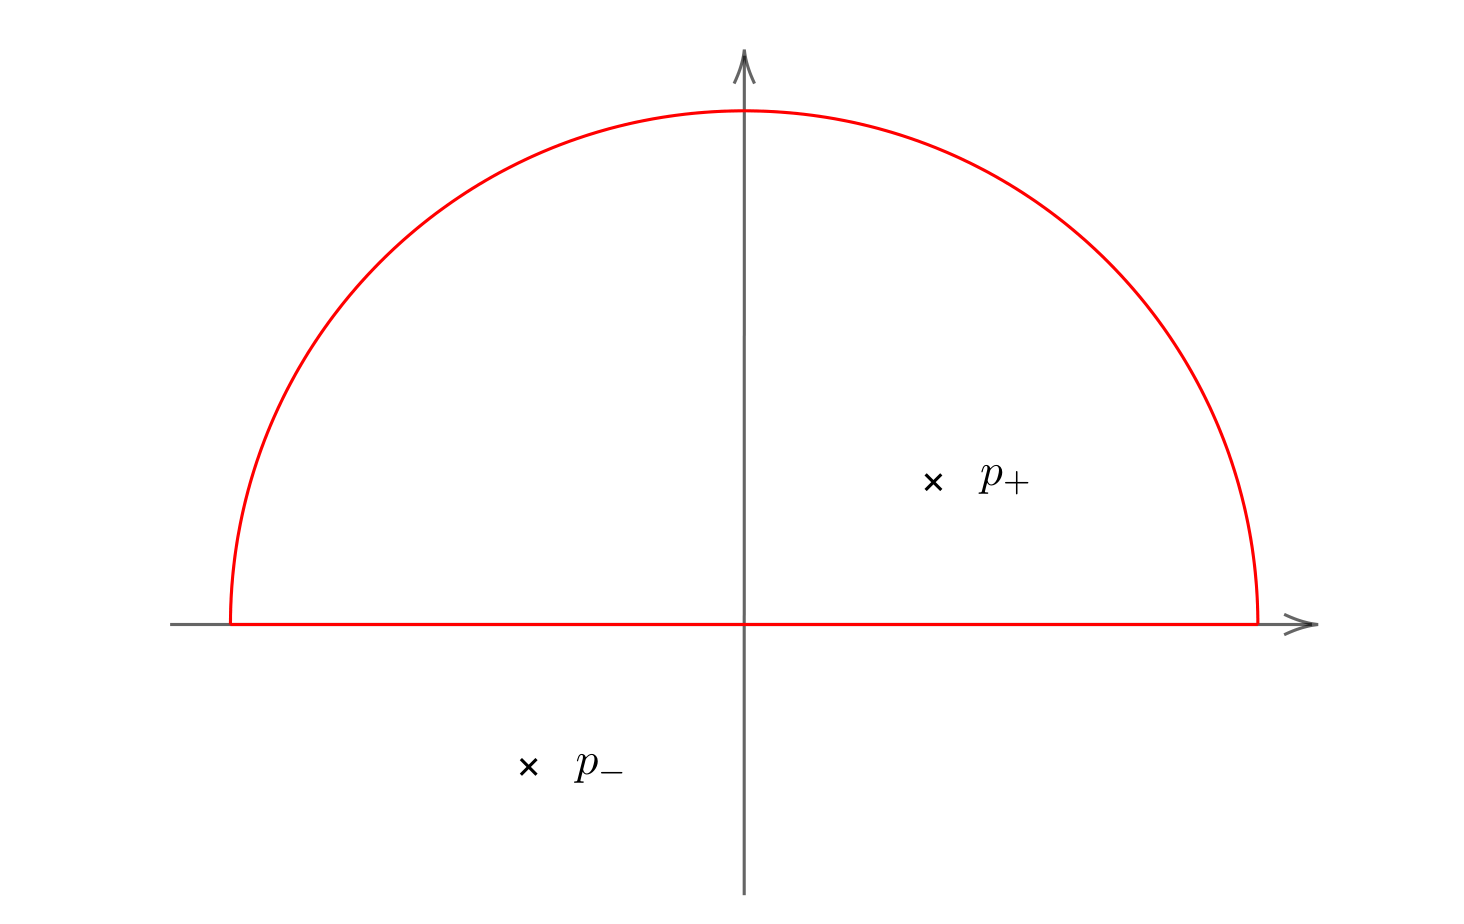
\includegraphics[width=0.65\textwidth]{figures/fig_p120_a.png}
\end{center}
% [图：原书 p.119，图内文字照原样保留]

  \[
  \begin{aligned}
  \Longrightarrow\quad G_0(x'',x';E)
  &=\frac{\ii}{\hs}\Res_{p=p_+}\left(
  \frac{\ee^{\ii p\abs{x''-x'}/\hs}}{E-p^2/2m+\ii\eps}
  \right)\qquad(\eps\to0_+)\\
  &=\frac1{\ii\hs}\sqrt{\frac{m}{2E}}\,
  \ee^{\ii\sqrt{2mE}\abs{x''-x'}/\hs}.
  \end{aligned}
  \]
  在物理区域 $E>0$、$E=\dfrac{\hs^2k^2}{2m}$（$k>0$）时，有
  \[
  G_0(x'',x';E)=\frac{m}{\ii\hs^2k}\ee^{\ii k\abs{x''-x'}}.
  \]
\end{example}

有一种构造格林函数的标准做法，我们针对眼前的情形简要回顾一下。设 $\psi_1(x)$ 与 $\psi_2(x)$ 是
\[
(E-\wh H)\psi_i(x)=0
\]
的两个线性无关解，即
\[
\left(\frac{\hs^2}{2m}\frac{\rd^2}{\rd x^2}-V(x)+E\right)\psi_i(x)=0.
\]
考虑如下函数
\[
\xi(x,y;E):=\frac{2m}{\hs^2W}
\left(\theta(x-y)\psi_1(x)\psi_2(y)+\theta(y-x)\psi_1(y)\psi_2(x)\right).
\]
这里 $W=\psi_1'(x)\psi_2(x)-\psi_2'(x)\psi_1(x)$ 称为\emph{朗斯基行列式}（Wronskian），由方程可知它是常数。利用 $\theta'(x-y)=\delta(x-y)$，可以直接验证 $\xi(x,y;E)$ 满足方程
\[
\left(\frac{\hs^2}{2m}\frac{\rd^2}{\rd x^2}-V(x)+E\right)\xi(x,y;E)=\delta(x-y).
\]
要使 $\xi(x,y;E)=G(x,y;E)$ 成立，我们需要选取 $\psi_1$ 与 $\psi_2$ 以满足适当的边界条件。我们在散射问题的例子中说明这一点。

\begin{example}{2.7.3}
  考虑
  \[
  \lim_{\abs{x}\to+\infty}V(x)=0
  \]
  的情形，它对散射问题是有意义的。考察傅里叶逆变换
  \[
  K(x'',T;x',0)=\frac{\ii}{2\pi}\int_{\R}\rd E\,
  \ee^{-\ii ET/\hs}G(x'',x';E).
  \]
  它可以看成来自不同能量的波函数的叠加。

  当 $x''\to+\infty$ 时，费曼核的行为应当像具有正动量、正能量的出射平面波。这说明
  \[
  G(x'',x';E)\propto\ee^{\frac{\ii}{\hs}\sqrt{2mE}\,x''}
  \qquad\text{当 }x''\to+\infty.
  \]
  类似地，$x''\to-\infty$ 时出射平面的行为说明
  \[
  G(x'',x';E)\propto\ee^{-\frac{\ii}{\hs}\sqrt{2mE}\,x''}
  \qquad\text{当 }x''\to-\infty.
  \]
  这导致解 $\psi_1$ 与 $\psi_2$ 的如下渐近行为
  \[
  \begin{cases}
  \psi_1(x)\propto\ee^{\frac{\ii}{\hs}\sqrt{2mE}\,x}, & x\to+\infty,\\[2mm]
  \psi_2(x)\propto\ee^{-\frac{\ii}{\hs}\sqrt{2mE}\,x}, & x\to-\infty.
  \end{cases}
  \]

% [原文 p.120]
  为说明这一点，考虑 $V=0$ 时的自由粒子。对 $E>0$，具有预期边界行为的解
  \[
  \left(\frac{\hs^2}{2m}\frac{\rd^2}{\rd x^2}+E\right)\psi_i(x)=0
  \]
  是
  \[
  \begin{cases}
  \psi_1(x)=\ee^{\ii kx},\\
  \psi_2(x)=\ee^{-\ii kx},
  \end{cases}
  \qquad
  k=\frac{\sqrt{2mE}}{\hs}.
  \]
  朗斯基行列式为 $W=\psi_1'\psi_2-\psi_1\psi_2'=2\ii k$。于是格林函数为
  \[
  \begin{aligned}
  G(x'',x';E)
  &=\frac{2m}{\hs^2\,2\ii k}
  \left(\theta(x''-x')\psi_1(x'')\psi_2(x')
  +\theta(x'-x'')\psi_1(x')\psi_2(x'')\right)\\
  &=\frac{m}{\ii\hs^2k}
  \left(\theta(x''-x')\ee^{\ii k(x''-x')}
  +\theta(x'-x'')\ee^{\ii k(x'-x'')}\right)\\
  &=\frac{m}{\ii\hs^2k}\ee^{\ii k\abs{x''-x'}},
  \end{aligned}
  \]
  它正是我们上面得到的公式。

  一般地，当局域势 $V(x)$ 打开时，我们处于散射过程的情形。考虑能量 $E>0$。于是行为
  \[
  \psi_1(x)\propto\ee^{\ii kx},\qquad x\to+\infty
  \]
  可以更精确地描述为
  \[
  \psi_1(x)=
  \begin{cases}
  \ee^{\ii kx}+B(k)\ee^{-\ii kx}, & x\to-\infty,\\[1mm]
  A(k)\ee^{\ii kx}, & x\to+\infty.
  \end{cases}
  \]

% [原文 p.121]
  这个解表示一列从 $x=-\infty$ 入射、穿过势区的平面波。系数 $B$ 表示反射波的振幅，$A$ 表示透射波的振幅。

  类似地，行为
  \[
  \psi_2(x)\propto\ee^{-\ii kx},\qquad x\to-\infty
  \]
  可以精确地描述为
  \[
  \psi_2(x)=
  \begin{cases}
  A(k)\ee^{-\ii kx}, & x\to-\infty,\\[1mm]
  \ee^{-\ii kx}+C(k)\ee^{\ii kx}, & x\to+\infty.
  \end{cases}
  \]
  这个解表示一列从 $x=+\infty$ 入射、穿过势区的平面波。系数 $C$ 表示反射波的振幅，$A$ 表示透射波的振幅。注意，由于时间反演对称性，从左方与从右方入射的透射振幅相同。

  我们可以由 $x=\pm\infty$ 处的行为计算朗斯基行列式，得到
  \[
  W=\psi_1'(x)\psi_2(x)-\psi_1(x)\psi_2'(x)=2\ii kA.
  \]
  于是格林函数为
  \[
  G(x'',x';E)=\frac{m}{\ii\hs^2kA}
  \left[\theta(x''-x')\psi_1(x'')\psi_2(x')
  +\theta(x'-x'')\psi_1(x')\psi_2(x'')\right].
  \]
  当 $x'\to-\infty$、$x''\to+\infty$ 时，得到
  \[
  G(x'',x';E)=\frac{m}{\ii\hs^2kA}A\,\ee^{\ii k(x''-x')},
  \qquad x'\to-\infty,\ x''\to+\infty,
  \]
  它显示了关于透射振幅的信息。在 §2.7.3 中，我们将用这个公式计算 $A$，并导出量子隧穿的 WKB 公式。
\end{example}

\subsection{半经典分析}

现在对格林函数
\[
G(x'',x';E)=\frac1{\ii\hs}\int_0^{\infty}\rd T\,
\ee^{\ii ET/\hs}K(x'',T;x',0)
\]
作半经典分析，取渐近极限 $\hs\to0$。回顾费曼核
\[
K(x'',T;x',0)=\int_{x(0)=x'}^{x(T)=x''}[\mathcal{D}x(t)]\,
\ee^{\frac{\ii}{\hs}S[x(t)]}.
\]
结合上述两式，得到
\[
G(x'',x';E)=\frac1{\ii\hs}\int_0^{\infty}\rd T\int[\mathcal{D}x(t)]\,
\ee^{\frac{\ii}{\hs}\left(ET+S[x(t)]\right)}.
\]
我们用最速下降法考虑 $\hs\to0$ 极限下的半经典近似。鞍点由 $(x_{cl},T_s)$ 给出，满足
\[
\begin{cases}
\left.\dfrac{\delta}{\delta x}\left(ET+S[x(t)]\right)\right|_{x(t)=x_{cl},T=T_s}=0,\\[3mm]
\left.\dfrac{\pa}{\pa T}\left(ET+S[x(t)]\right)\right|_{x(t)=x_{cl},T=T_s}=0.
\end{cases}
\]

% [原文 p.122]
第一式即
\[
\left.\frac{\delta S}{\delta x}\right|_{x=x_{cl},T=T_s}=0,
\]
也就是说，$x_{cl}(t)$ 是一条从 $x_{cl}(0)=x'$ 到 $x_{cl}(T_s)=x''$ 的经典轨迹。把 $x_{cl}$ 代入第二式，并利用哈密顿–雅可比方程，得到
\[
E=-\frac{\pa S[x_{cl}]}{\pa T}=E_{cl}.
\]
这里 $E_{cl}$ 是经典轨迹 $x_{cl}$ 的能量。因此，鞍点是满足下述条件的数对 $(x_{cl},T_s)$ 的集合：$x_{cl}$ 是一条从 $x'$ 到 $x''$、能量为 $E$、耗时为 $T_s$ 的经典轨迹。

现在计算鞍点 $(x_{cl},T_s)$ 处的半经典贡献。记 $S_{cl}$ 为经典轨迹 $x_{cl}$ 上的作用量 $S[x_{cl}]$。回忆费曼核的如下半经典近似
\[
K_{sc}(x'',T;x',0)=
\left(\frac{\ii}{2\pi\hs}\frac{\pa^2 S_{cl}}{\pa x''\pa x'}\right)^{\frac12}
\ee^{\frac{\ii}{\hs}S_{cl}}.
\]
由此得到 $\hs\to0$ 极限下格林函数的如下半经典渐近行为
\[
\begin{aligned}
G(x'',x';E)
&\simeq\sum_{(x_{cl},T_s)}\frac1{\ii\hs}
\left(\frac{\ii}{2\pi\hs}\frac{\pa^2 S_{cl}}{\pa x''\pa x'}\right)^{\frac12}
\left(\frac{2\pi\hs\ii}{\pa_T^2 S_{cl}}\right)^{\frac12}
\ee^{\frac{\ii}{\hs}(ET_s+S_{cl})}\\
&=\frac1{\hs}\sum_{(x_{cl},T_s)}
\left(\frac{\dfrac{\pa^2 S_{cl}}{\pa x''\pa x'}}
{-\dfrac{\pa E_{cl}}{\pa T}}\right)^{\frac12}
\ee^{\frac{\ii}{\hs}(ET_s+S_{cl})}.
\end{aligned}
\]
这个表达式还可以进一步化简。回忆 §2.6.2 中的
\[
\frac{\pa^2 S_{cl}}{\pa x''\pa x'}=-\frac{m}{J(T)},
\]
其中 $J$ 是沿轨迹求解
\[
\begin{cases}
\left(\dfrac{\rd^2}{\rd t^2}+\dfrac1m V''(x_{cl}(t))\right)J(t)=0,\\[2mm]
J(0)=0,\qquad \dot J(0)=1
\end{cases}
\]
的雅可比场。记 $v_{cl}(t)=\dot x_{cl}(t)$ 为沿轨迹的速度。把轨迹方程
\[
m\ddot x_{cl}(t)+V'(x_{cl}(t))=0
\]
关于 $t$ 求导，得到
\[
\left(\frac{\rd^2}{\rd t^2}+\frac1m V''(x_{cl}(t))\right)v_{cl}(t)=0,
\]
即 $v_{cl}(t)$ 与 $J$ 满足同一个方程。

由于 $v_{cl}(t)$ 与轨迹相切，而 $J(t)$ 沿法向，$\{v,J\}$ 构成该方程的两个线性无关解。朗斯基行列式
\[
W=\dot J(t)v_{cl}(t)-J(t)\dot v_{cl}(t)
\]

% [原文 p.123]
由方程可知是常数。在 $t=0$ 处计算 $W$，得到 $W=v_{cl}(0)$。于是
\[
\frac{\rd}{\rd t}\left(\frac{J(t)}{v_{cl}(t)}\right)
=\frac{W}{v_{cl}(t)^2}=\frac{v_{cl}(0)}{v_{cl}(t)^2}
\quad\Longrightarrow\quad
J(T)=v_{cl}(0)v_{cl}(T)\int_0^T\frac{\rd t}{v_{cl}(t)^2}.
\]
另一方面，
\[
T=\int_0^T\rd t=\int_{x'}^{x''}\frac{\rd x}{v_{cl}(t)}
=\int_{x'}^{x''}\frac{\rd x}{\sqrt{2(E_{cl}-V(x))/m}},
\]
\[
\Longrightarrow\quad
\frac{\rd T}{\rd E_{cl}}
=-\frac1m\int_{x'}^{x''}
\frac{\rd x}{(2(E_{cl}-V(x))/m)^{3/2}}
=-\frac1m\int_{x'}^{x''}\frac{\rd x}{v_{cl}^3}
=-\frac1m\int_0^T\frac{\rd t}{v_{cl}(t)^2},
\]
\[
\Longrightarrow\quad
\frac{\pa E_{cl}}{\pa T}
=-\frac{m}{\displaystyle\int_0^T\frac{\rd t}{v_{cl}(t)^2}}.
\]
由此可知
\[
\frac{\dfrac{\pa^2 S_{cl}}{\pa x''\pa x'}}{-\dfrac{\pa E_{cl}}{\pa T}}
=\frac{-\dfrac{m}{J(T)}}{
\dfrac{m}{\int_0^T\frac{\rd t}{v_{cl}(t)^2}}}
=\frac1{-v_{cl}(0)v_{cl}(T)}
=\frac1{-\dot x_{cl}(0)\dot x_{cl}(T)}.
\]
我们再定义 $W_{cl}=E_{cl}T_s+S_{cl}$。则
\[
\begin{aligned}
W_{cl}
&=E_{cl}T_s+\int_0^{T_s}\left(\frac{m}{2}\dot x_{cl}^2-V(x_{cl})\right)\rd t\\
&=E_{cl}T_s+\int_0^{T_s}m\dot x_{cl}^2\,\rd t-\int_0^{T_s}E_{cl}\,\rd t\\
&=\int_0^{T_s}m\dot x_{cl}^2\,\rd t=\int_{x'}^{x''}p\,\rd x.
\end{aligned}
\]
这里 $p=m\dot x=\sqrt{2m(E-V(x))}$ 是经典动量。于是我们得到如下渐近半经典近似
\[
\begin{aligned}
G(x',x'';E)
&\simeq\frac1{\hs}\sum_{(x_{cl},T_s)}
\left(-\dot x_{cl}(0)\dot x_{cl}(T_s)\right)^{-\frac12}
\ee^{\frac{\ii}{\hs}W_{cl}}\\
&=\frac1{\hs}\sum_{(x_{cl},T_s)}
\left(-\dot x_{cl}(0)\dot x_{cl}(T_s)\right)^{-\frac12}
\ee^{\frac{\ii}{\hs}\int_{x'}^{x''}p\,\rd x}.
\end{aligned}
\]

\begin{remark}{2.7.4}
  这里有一点值得强调。由于 $T$ 的积分围道是
  \[
  \int_0^{\infty}\rd T,
  \]
  我们并不是对所有可能的经典轨迹 $(x_{cl},T_s)$ 求和。事实上，为了应用最速下降法，我们必须把积分围道
  \[
  \int_0^{\infty}\rd T=\int_C\rd T
  \]
  从 $\R_{\ge0}$ 形变到由最速下降曲线组合而成的围道 $C$。随着参数 $x',x''$ 的变化，这些最速下降曲线的和可能出现不连续的跳跃。这正是斯托克斯现象。
\end{remark}

% [原文 p.124]
\begin{example}{2.7.5（自由粒子）}
  给定能量 $E>0$，存在唯一的经典轨迹从 $x'$ 到 $x''$：
  \[
  x_{cl}(t)=x'+\frac{x''-x'}{T_s}t,
  \]
  其中
  \[
  T_s=\sqrt{\frac{m}{2E}}\abs{x''-x'}.
  \]
  半经典格林函数为
  \[
  \begin{aligned}
  G(x',x'';E)
  &\simeq\frac1{\hs}\left(-\dot x_{cl}(0)\dot x_{cl}(T_s)\right)^{-\frac12}
  \ee^{\frac{\ii}{\hs}\int_{x'}^{x''}p_{cl}\,\rd x_{cl}}\\
  &=\frac1{\hs}\left(-\frac{2E}{m}\right)^{-\frac12}
  \ee^{\frac{\ii}{\hs}\sqrt{2mE}\abs{x''-x'}}\\
  &=\frac{m}{\ii\hs^2k}\ee^{\ii k\abs{x''-x'}},
  \qquad k=\frac{\sqrt{2mE}}{\hs}.
  \end{aligned}
  \]
  这与我们先前得到的公式相同。
\end{example}

\begin{example}{2.7.6（线性势）}
  我们考虑线性势
  \[
  V(x)=-\lambda x,\qquad \lambda>0
  \]
  的例子。

  这个例子在推导 WKB 近似的连接公式时起着重要作用。我们将在 §2.7.3 中通过半经典路径积分理解连接公式的不同视角。这里先按文献 [9] 的讲述说明基本想法。

  运动方程为
  \[
  m\ddot x=\lambda.
  \]
  给定 $T$，存在唯一的经典轨迹从 $x(0)=x'$ 到 $x(T)=x''$：
  \[
  x_{cl}(t)=x'+\frac{x''-x'}{T}t-\frac{\lambda T}{2m}t+\frac{\lambda}{2m}t^2.
  \]
  相应的作用量值为
  \[
  S_{cl}=\int_0^T\left(\frac12 m\dot x_{cl}^2+\lambda x_{cl}\right)\rd t
  =\frac{m}{2T}(x''-x')^2+\frac{\lambda T}{2}(x''+x')-\frac{\lambda^2T^3}{24m}.
  \]
  在线性情形，半经典费曼核是精确的：
  \[
  K(x'',T;x',0)=
  \left(\frac{\ii}{2\pi\hs}\frac{\pa^2 S_{cl}}{\pa x''\pa x'}\right)^{\frac12}
  \ee^{\frac{\ii}{\hs}S_{cl}}
  =\left(\frac{m}{2\pi\ii\hs T}\right)^{\frac12}
  \ee^{\frac{\ii}{\hs}S_{cl}}.
  \]

  现在我们考虑格林函数 $G(x'',x';E)$ 沿 $T$ 积分时的鞍点。注意，对线性势，能量的平移等价于 $x$ 的平移。因此只需考虑 $E=0$ 的情形，此时
  \[
  W_{cl}=S_{cl}.
  \]
  在下面的讨论中我们假设 $E=0$。

% [原文 p.125]
  鞍点 $(x_{cl},T_s)$ 位于时刻 $T_s$，由
  \[
  E=-\left.\frac{\pa S_{cl}}{\pa T}\right|_{T=T_s}
  \]
  给出，即
  \[
  \Longrightarrow\quad
  \frac{m}{2T_s^2}(x''-x')^2-\frac{\lambda}{2}(x''+x')+\frac{\lambda^2T_s^2}{8m}=0,
  \]
  \[
  \Longrightarrow\quad
  T_s=\left(\frac{2m}{\lambda}\right)^{\frac12}
  \left(\pm\sqrt{x''}\pm\sqrt{x'}\right).
  \]
  总共有四个鞍点，对应于 $\sqrt{x'}$ 与 $\sqrt{x''}$ 取平方根时所有可能的符号选择。经典作用量的值为
  \[
  S_{cl}=\frac23(2m\lambda)^{\frac12}
  \left(\pm\sqrt{x''}^3\pm\sqrt{x'}^3\right),
  \]
  其中 $\sqrt{x''}$ 与 $\sqrt{x'}$ 的符号与 $T_s$ 中的一致。初速度与末速度之积为
  \[
  \begin{aligned}
  \dot x_{cl}(0)\dot x_{cl}(T_s)
  &=\left(\frac{x''-x'}{T_s}-\frac{\lambda T_s}{2m}\right)
  \left(\frac{x''-x'}{T_s}+\frac{\lambda T_s}{2m}\right)\\
  &=\frac{(x''-x')^2}{T_s^2}-\frac{\lambda^2}{4m^2}T_s^2\\
  &=\frac{\lambda}{m}(x''+x')-\frac{\lambda^2}{2m^2}T_s^2\\
  &=-\frac{2\lambda}{m}\left(\pm\sqrt{x''}\right)\left(\pm\sqrt{x'}\right).
  \end{aligned}
  \]
  于是鞍点 $(x_{cl},T_s)$ 对格林函数的半经典贡献为
  \[
  \frac1{\hs}
  \left(\frac{m}{2\lambda\left(\pm\sqrt{x''}\right)\left(\pm\sqrt{x'}\right)}
  \right)^{\frac12}\ee^{\frac{\ii}{\hs}S_{cl}}.
  \]

  现在我们来判断哪些鞍点会对半经典格林函数作出贡献。情形取决于 $x'$ 与 $x''$ 的位置。

  \textbf{情形 $0<x'<x''$}

  $x'$ 与 $x''$ 都位于经典允许区（$x>0$）内。

% [原文 p.126]
  \begin{center}
  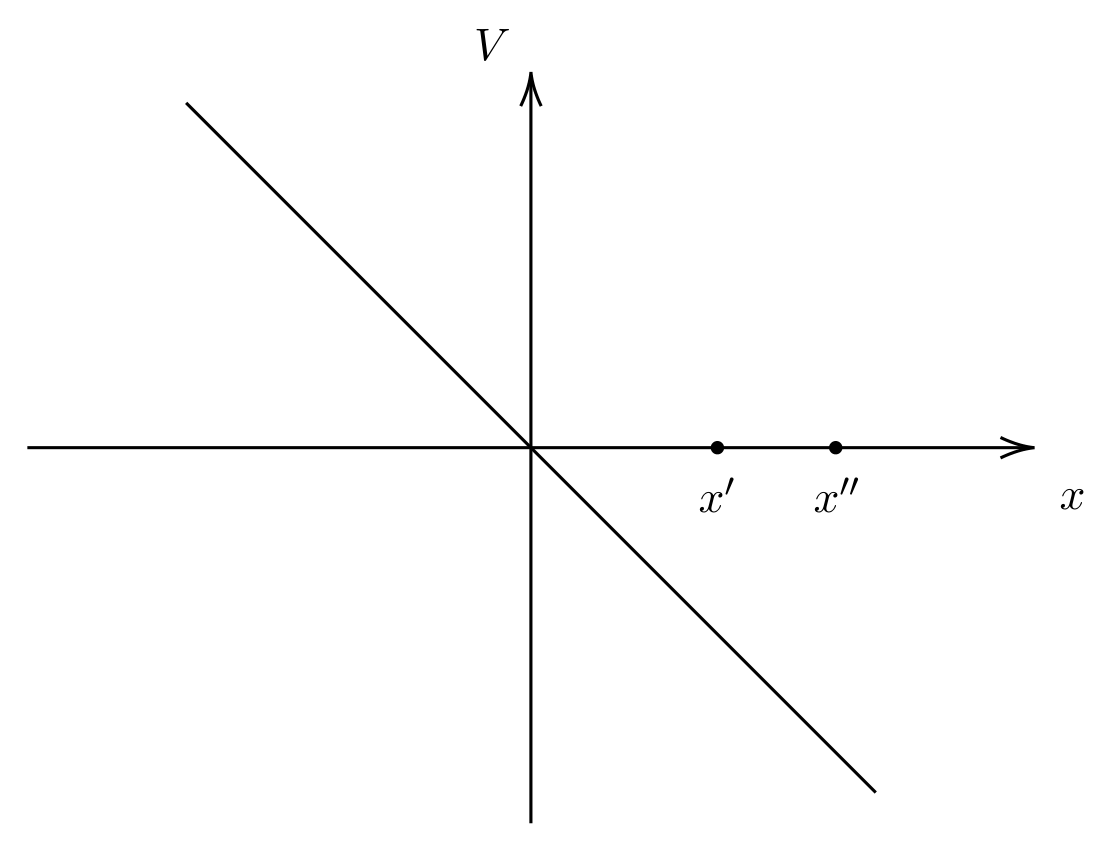
\includegraphics[width=0.6\textwidth]{figures/fig_p126_a.png}
  \end{center}
  % [图：原书 p.125，图内文字照原样保留]

所有鞍点都取实值，我们记为
\[
T_s^{(\pm\pm)}=\left(\frac{2m}{\lambda}\right)^{\frac12}
\left(\pm\sqrt{x'}\pm\sqrt{x''}\right).
\]

\begin{center}
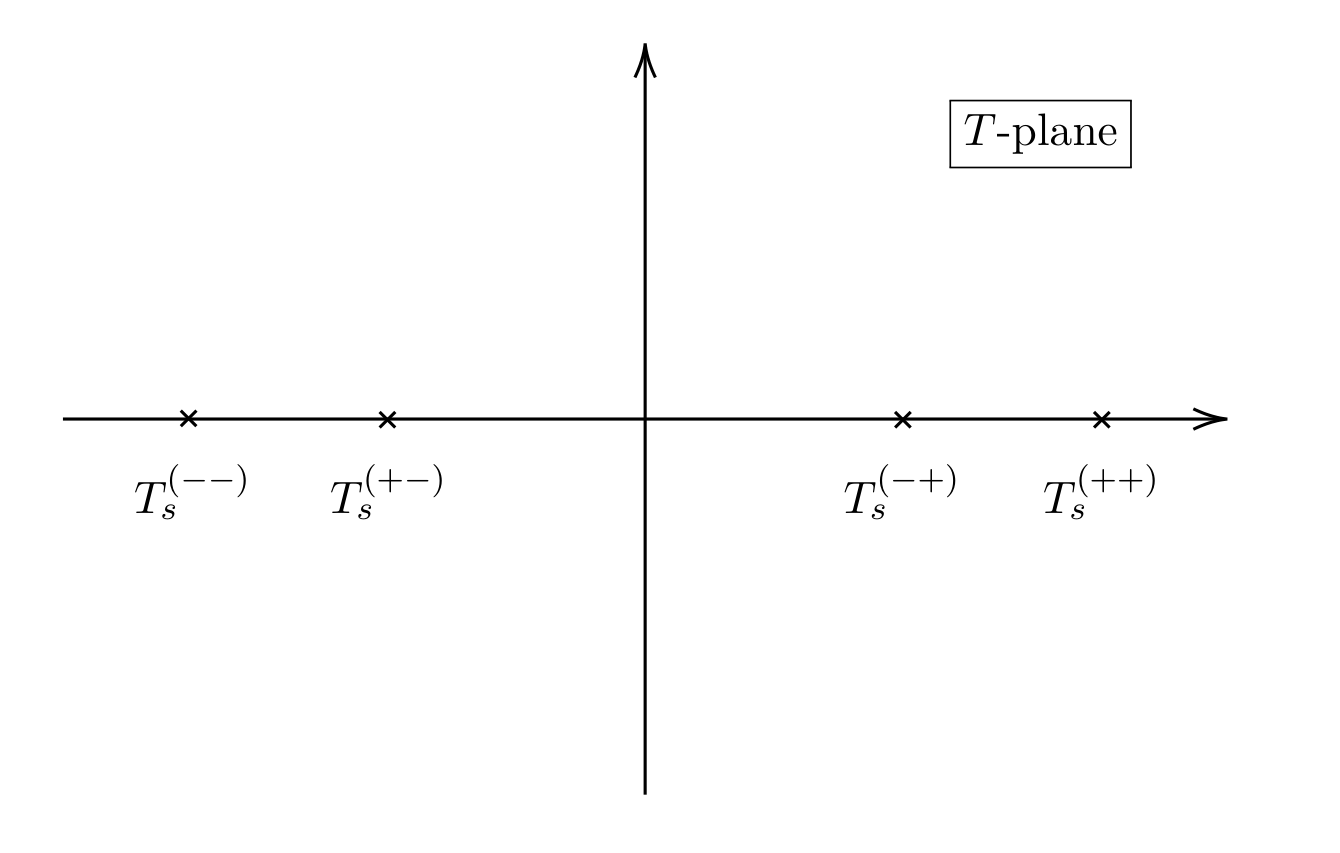
\includegraphics[width=0.62\textwidth]{figures/fig_p127_a.png}
\end{center}
% [图：原书 p.126，图内文字照原样保留]

考虑 $T$ 平面中的最速下降曲线。所考察的复振荡积分涉及函数（此处 $E=0$）
\[
\ee^{\frac{\ii}{\hs}(ET+S_{cl})}=\ee^{\frac{\ii}{\hs}S_{cl}}.
\]
$T$ 平面中的最速下降曲线由以下条件描述：
\begin{itemize}
\item $\Imag(\ii S_{cl})=\Real(S_{cl})=\text{常数}$；
\item $\Real(\ii S_{cl})=-\Imag(S_{cl})\to-\infty$（沿边界）；
\item 经过某个鞍点。
\end{itemize}

经典作用量 $S_{cl}$ 作为 $T$ 的函数为
\[
S_{cl}(T)=\frac{m}{2T}(x''-x')^2+\frac{\lambda T}{2}(x''+x')
-\frac{\lambda^2T^3}{24m}.
\]
$S_{cl}$ 在 $T_s^{(\pm\pm)}$ 处的相应值为
\[
S_{cl}\left(T_s^{(\pm\pm)}\right)
=\frac23(2m\lambda)^{\frac12}\left(\pm\sqrt{x'}^3\pm\sqrt{x''}^3\right).
\]
于是所有 $\Real\left(S_{cl}\left(T_s^{(\pm\pm)}\right)\right)$ 互不相同，相应的四条最速下降曲线 $C^{(\pm\pm)}$ 互不相交。它们可以通过沿 $u\to+\infty$ 的流方程来构造
\[
\frac{\rd T}{\rd u}=-\ii\,\ol{S_{cl}'(T)},
\]
即
\[
\frac{\rd T}{\rd u}=\ii\left[-\frac{m}{2\ol T^2}(x''-x')^2
+\frac{\lambda}{2}(x''+x')-\frac{\lambda^2\ol T^2}{8m}\right],
\]
初值条件为 $\lim\limits_{u\to-\infty}T=\text{鞍点}$。

% [原文 p.127]
现在把 §2.5.3 的方法用于
\[
f(T)=\ii S_{cl}(T).
\]
我们有
\[
S_{cl}'(T)=-\frac{\lambda^2}{8mT^2}
\left(T-T_s^{(--)}\right)\left(T-T_s^{(+-)}\right)
\left(T-T_s^{(-+)}\right)\left(T-T_s^{(++)}\right).
\]
在四个鞍点处，$S_{cl}''$ 的符号依次为：$T_s^{(--)}$ 处 $S_{cl}''>0$，$T_s^{(+-)}$ 处 $S_{cl}''<0$，$T_s^{(-+)}$ 处 $S_{cl}''>0$，$T_s^{(++)}$ 处 $S_{cl}''<0$。

于是可以画出每个鞍点处最速下降曲线的切方向：
\begin{center}
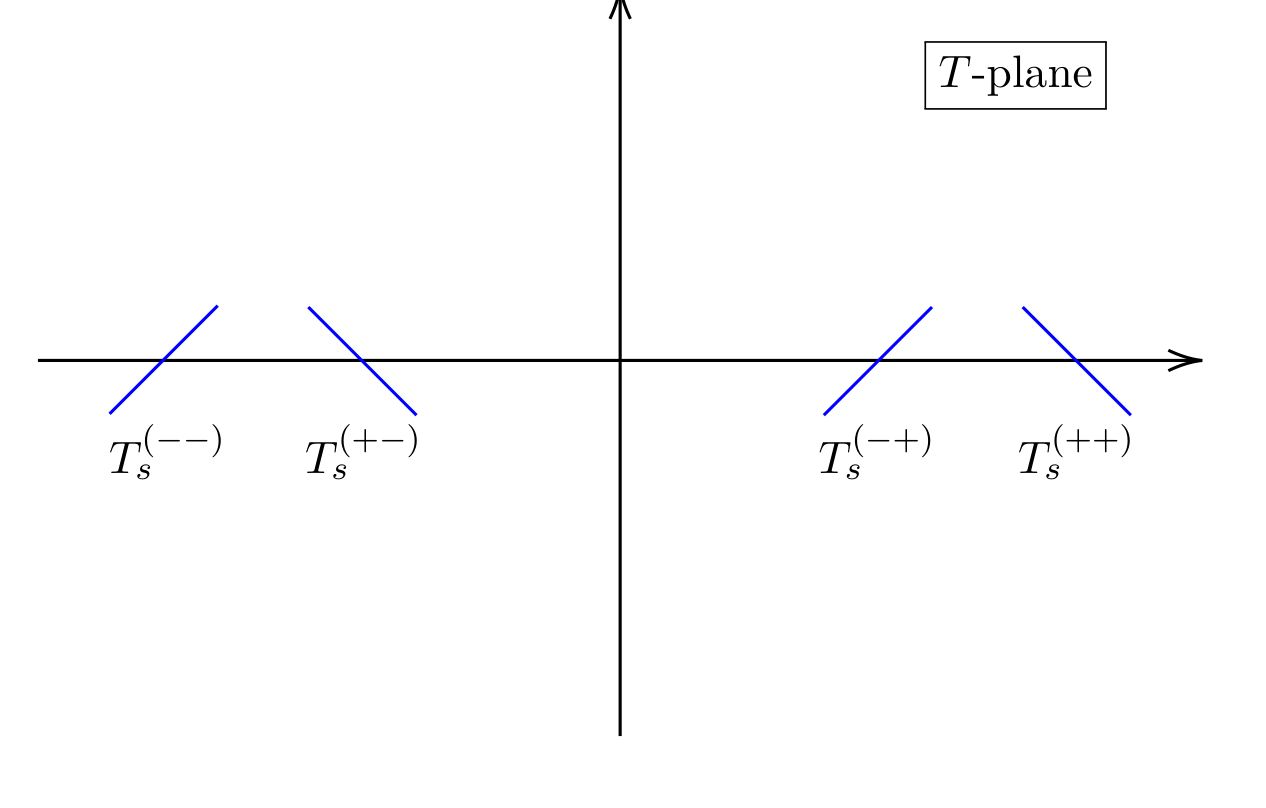
\includegraphics[width=0.66\textwidth]{figures/fig_p128_a.png}
\end{center}
% [图：原书 p.127，图内文字照原样保留]

再作一些计算可知，积分围道 $\{T\in\R_{\ge0}\}$ 形变为如下两条最速下降曲线之和：
\begin{center}
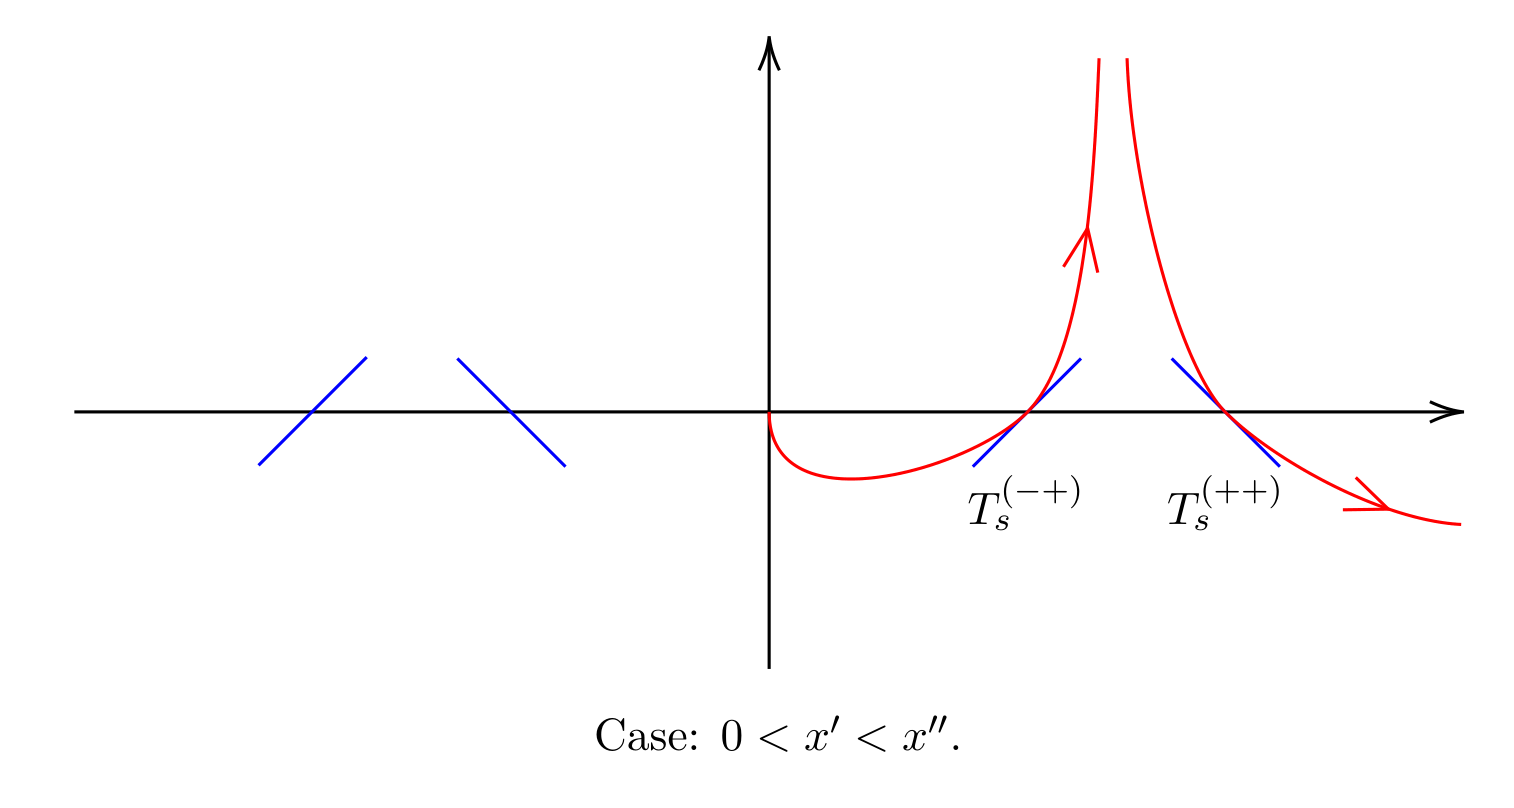
\includegraphics[width=0.72\textwidth]{figures/fig_p128_b.png}
\end{center}
% [图：原书 p.127，图内文字照原样保留]
\nopagebreak[4]
\fignote{图内文字：Case: $0<x'<x''$（情形：$0<x'<x''$）}

于是格林函数 $G(x'',x';E)$ 的半经典近似只来自两个鞍点的贡献
\[
T_s^{(-+)}=\left(\frac{2m}{\lambda}\right)^{\frac12}
\left(-\sqrt{x'}+\sqrt{x''}\right),
\]

% [原文 p.128]
\[
T_s^{(++)}=\left(\frac{2m}{\lambda}\right)^{\frac12}
\left(\sqrt{x'}+\sqrt{x''}\right).
\]
鞍点 $T_s^{(-+)}$ 对应从 $x'$ 到 $x''$ 的直达路径。另一个鞍点 $T_s^{(++)}$ 对应的路径从 $x'$ 出发向左运动，在 $x=0$ 处反射，然后向右运动到达 $x''$。

\noindent\textbf{情形 $x'<0<x''$}

$x'$ 位于经典禁区，$x''$ 位于经典允许区。
\begin{center}
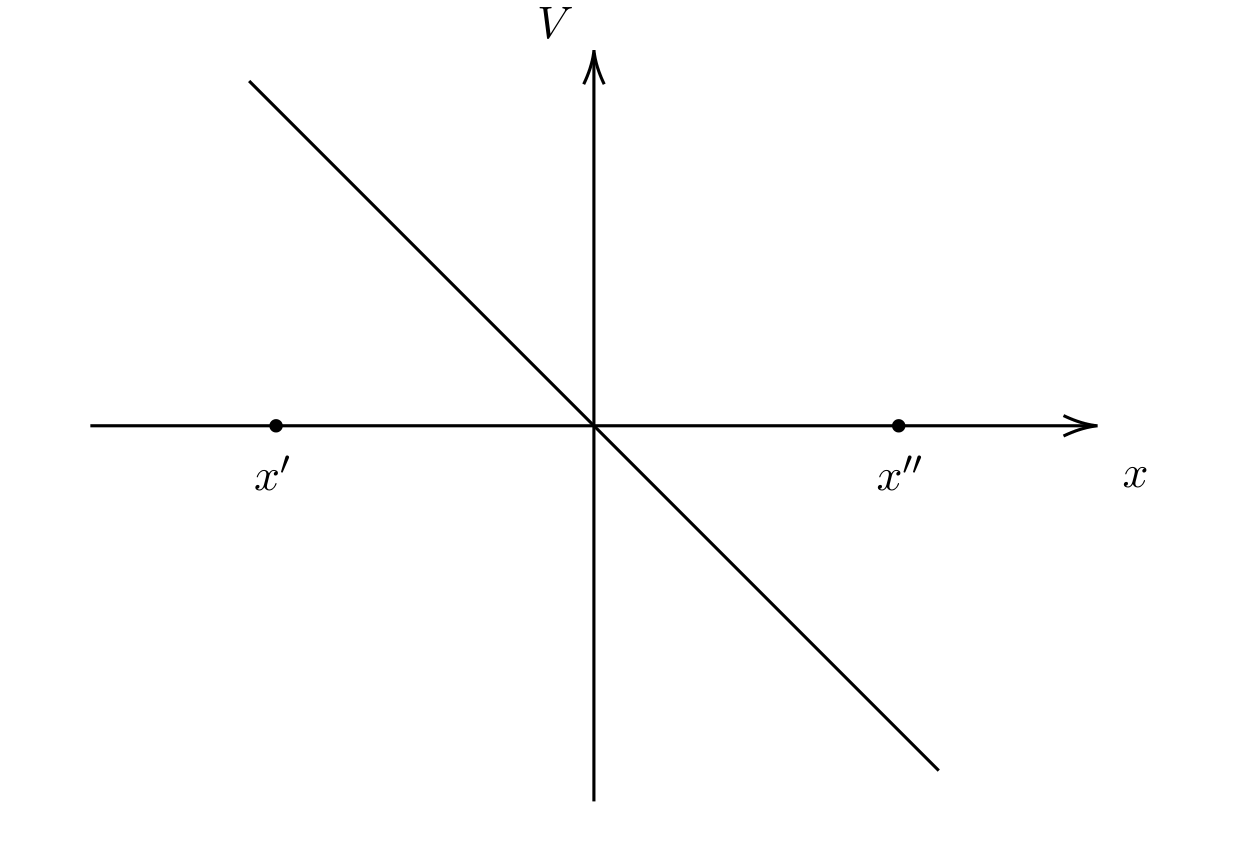
\includegraphics[width=0.6\textwidth]{figures/fig_p129_a.png}
\end{center}
% [图：原书 p.128，图内文字照原样保留]

四个鞍点
\[
T_s^{(\pm\pm)}=\left(\frac{2m}{\lambda}\right)^{\frac12}
\left(\pm\ii\sqrt{|x'|}\pm\sqrt{x''}\right)
\]
都是复数。
\begin{center}
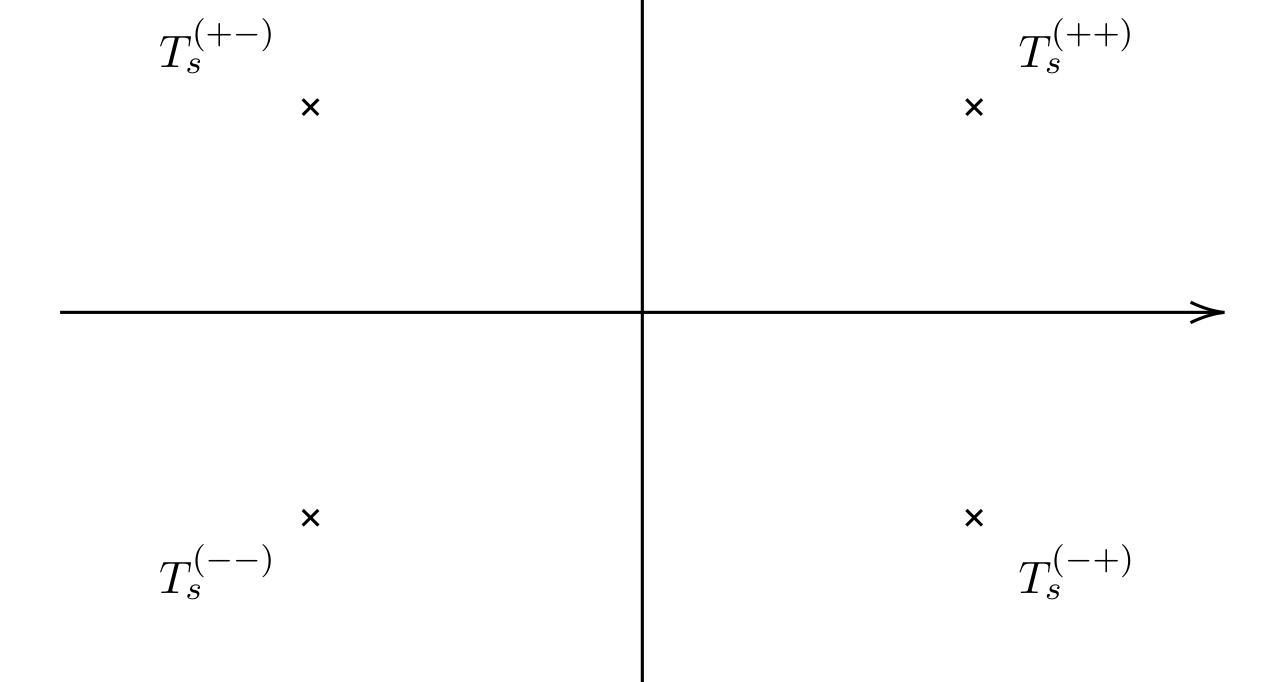
\includegraphics[width=0.62\textwidth]{figures/fig_p129_b.png}
\end{center}
% [图：原书 p.128，图内文字照原样保留]

\[
S_{cl}'(T)=-\frac{\lambda^2}{8mT^2}
\left(T-T_s^{(--)}\right)\left(T-T_s^{(+-)}\right)
\left(T-T_s^{(-+)}\right)\left(T-T_s^{(++)}\right).
\]

% [原文 p.129]
在鞍点处有
\[
\begin{aligned}
\ii S_{cl}''\left(T_s^{(++)}\right)&\in\left(T_s^{(++)}\right)^{-1}\R_{>0},\\
\ii S_{cl}''\left(T_s^{(+-)}\right)&\in-\left(T_s^{(+-)}\right)^{-1}\R_{>0},\\
\ii S_{cl}''\left(T_s^{(-+)}\right)&\in-\left(T_s^{(-+)}\right)^{-1}\R_{>0},\\
\ii S_{cl}''\left(T_s^{(--)}\right)&\in\left(T_s^{(--)}\right)^{-1}\R_{>0}.
\end{aligned}
\]
由此可以画出鞍点处最速下降曲线的切方向。
\begin{center}
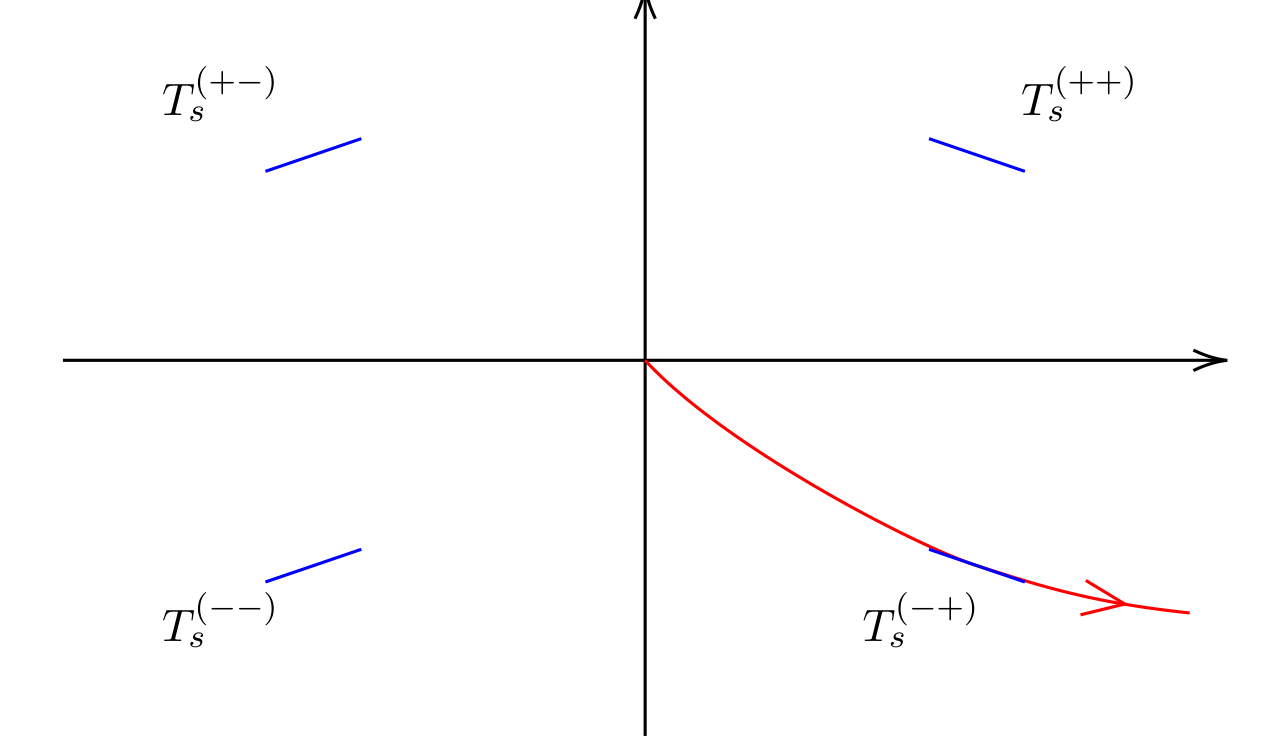
\includegraphics[width=0.62\textwidth]{figures/fig_p130_a.png}
\end{center}
% [图：原书 p.129，图内文字照原样保留]

积分围道 $\{T\in\R_{\ge0}\}$ 形变为过
\[
T_s^{(-+)}=\left(\frac{2m}{\lambda}\right)^{\frac12}
\left(-\ii\sqrt{|x'|}+\sqrt{x''}\right)
\]
的最速下降曲线。

注意鞍点 $T_s^{(-+)}$ 有虚部。它对应从 $x'$ 到 $x''$ 的唯一经典路径，但这条路径必须经过非实的时间！这个非实时间源于以下事实：路径必须穿过一段经典禁区。确实，
\[
T=\int_0^T\rd t=\int_{x'}^{x''}\frac{\rd x}{\dot x}
=\int_{x'}^{x''}\frac{\rd x}{\sqrt{2m(E-V(x))}}.
\]
在经典禁区中 $E<V(x)$，因此该积分给出旅行时间的虚贡献。

\noindent\textbf{情形 $x'<x''<0$}

$x'$ 与 $x''$ 都位于禁区。

% [原文 p.130]
\begin{center}
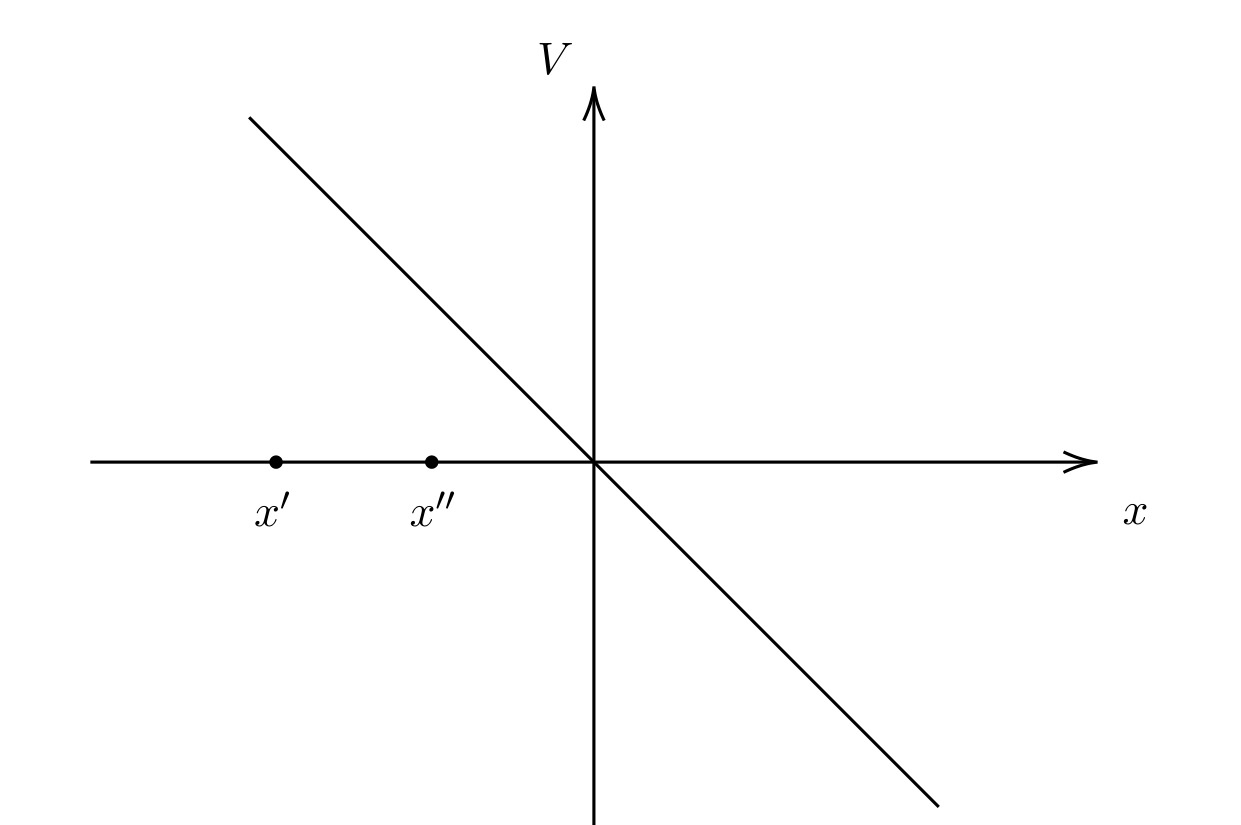
\includegraphics[width=0.6\textwidth]{figures/fig_p131_a.png}
\end{center}
% [图：原书 p.130，图内文字照原样保留]

四个鞍点
\[
T_s^{(\pm\pm)}=\left(\frac{2m}{\lambda}\right)^{\frac12}
\left(\pm\ii\sqrt{|x'|}\pm\ii\sqrt{|x''|}\right)
\]
都是纯虚数。
\begin{center}
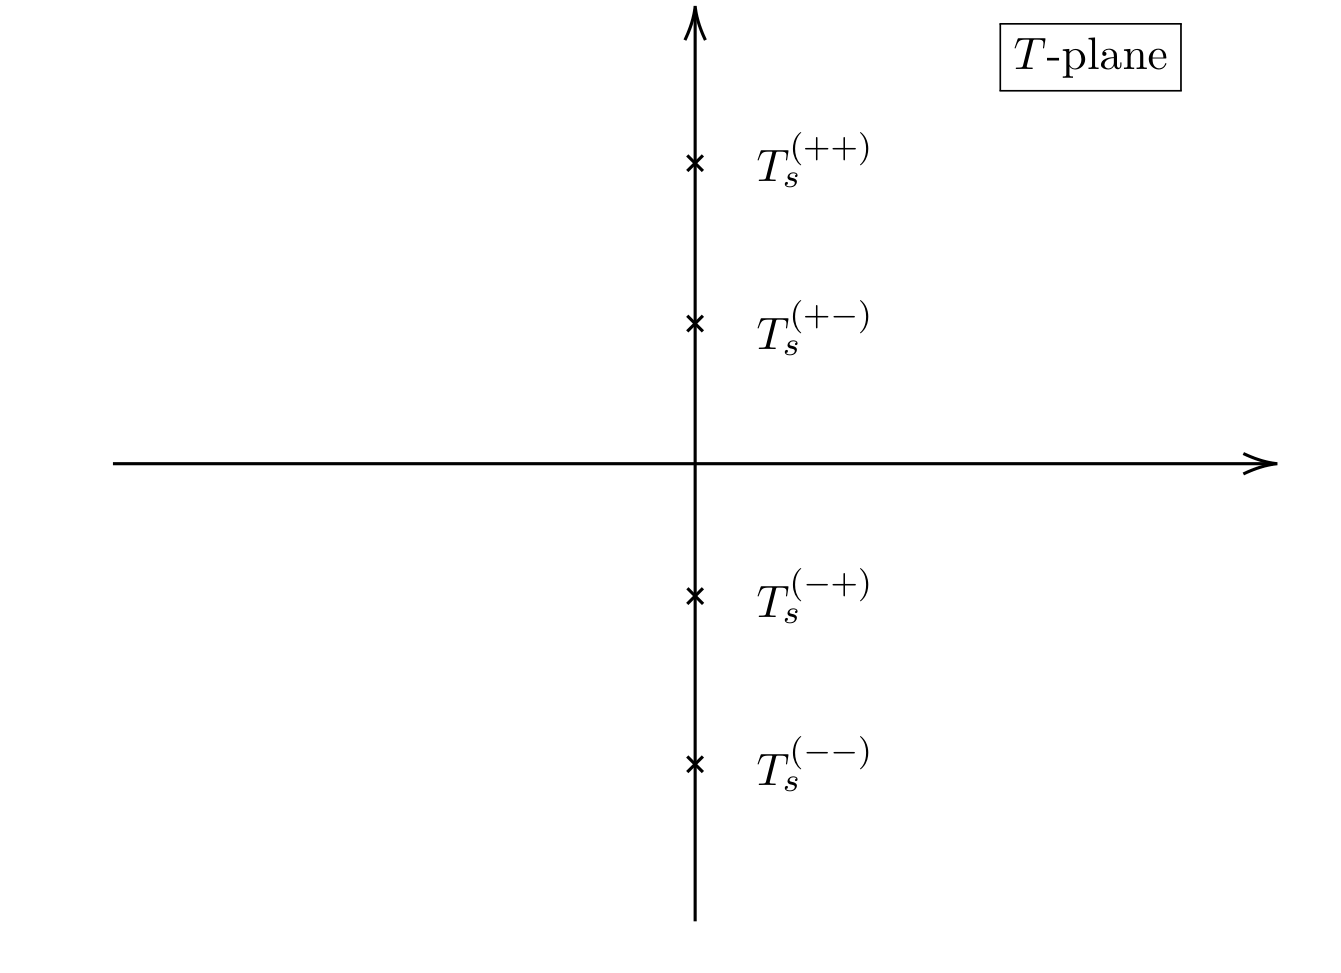
\includegraphics[width=0.6\textwidth]{figures/fig_p131_b.png}
\end{center}
% [图：原书 p.130，图内文字照原样保留]

在鞍点处有
\[
\begin{aligned}
\ii S_{cl}''\left(T_s^{(++)}\right)&\in\R_{>0},\\
\ii S_{cl}''\left(T_s^{(+-)}\right)&\in\R_{<0},\\
\ii S_{cl}''\left(T_s^{(-+)}\right)&\in\R_{>0},\\
\ii S_{cl}''\left(T_s^{(--)}\right)&\in\R_{<0}.
\end{aligned}
\]
由此可以画出鞍点处最速下降曲线的切方向。

% [原文 p.131]
\begin{center}
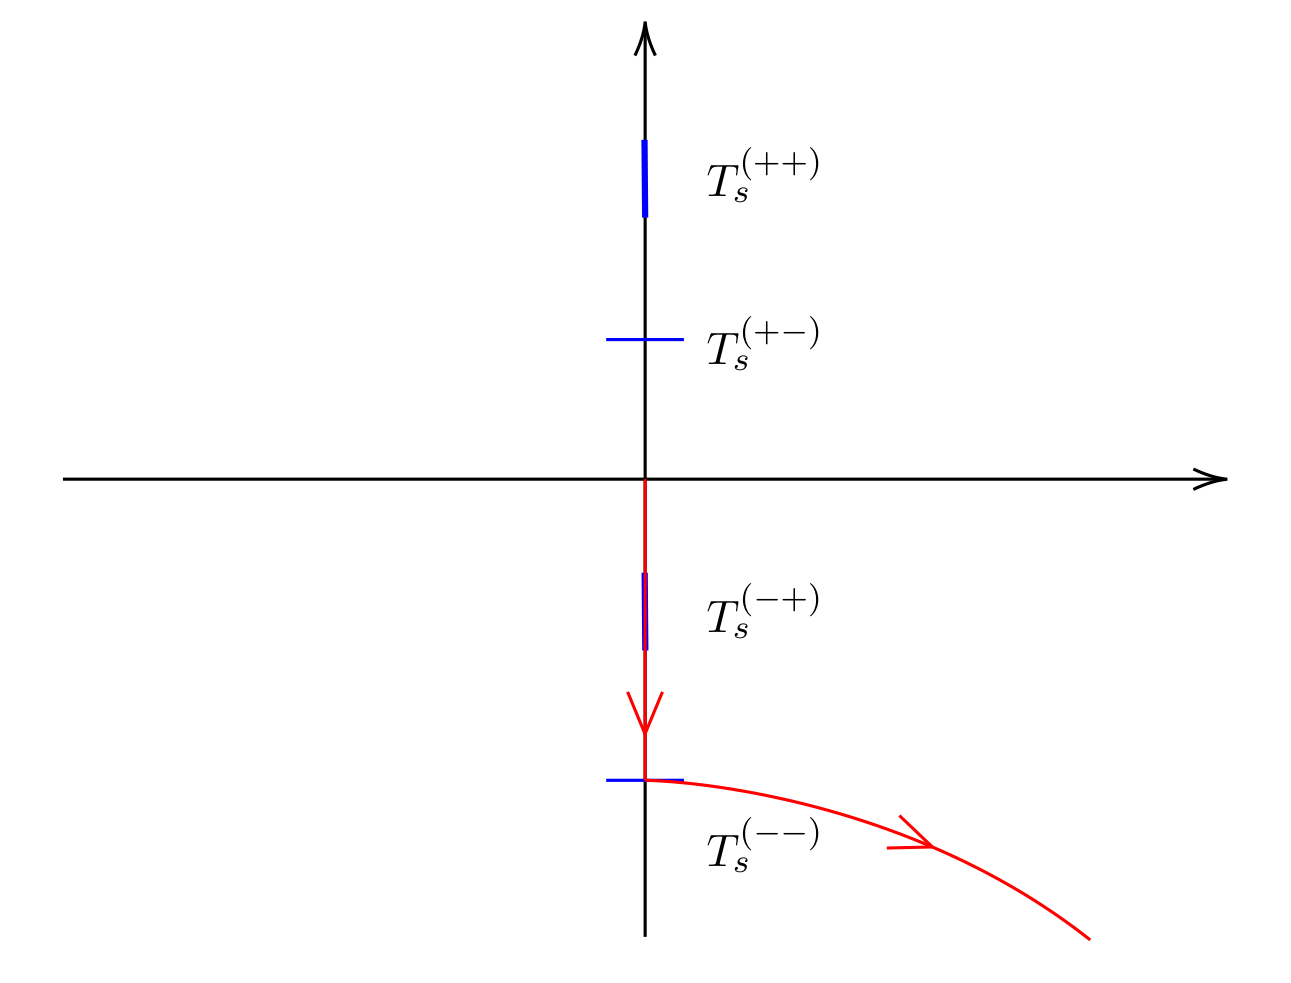
\includegraphics[width=0.62\textwidth]{figures/fig_p132_a.png}
\end{center}
% [图：原书 p.131，图内文字照原样保留]

积分围道 $\{T\in\R_{\ge0}\}$ 形变为两条分别过 $T_s^{(-+)}$ 与 $T_s^{(--)}$ 的曲线。第一条曲线从原点出发，经过鞍点 $T_s^{(-+)}$，终止于鞍点 $T_s^{(--)}$。第二条曲线从鞍点 $T_s^{(--)}$ 出发，走向无穷远。鞍点 $T_s^{(-+)}$ 的贡献占主导。
\end{example}

\subsection{经由路径积分的 WKB}

现在把路径积分的半经典近似，与波函数的半经典近似（WKB 形式）联系起来。

格林函数
\[
G(x'',x';E)=\bra{x''}\frac{1}{E-\wh H}\ket{x'}
\]
是算子 $E-\wh H$ 的逆核，并且满足
\[
\left(E-\wh H_{x''}\right)G(x'',x';E)=\delta(x''-x').
\]
这里 $\wh H_{x''}$ 是用 $x''$-坐标表示的哈密顿算子。

在上一小节中，我们证明了渐近的半经典公式
\[
G(x'',x';E)\simeq\frac{1}{\hs}
\sum_{(x_{cl},T_s)}\left(-\dot x_{cl}(0)\dot x_{cl}(T_s)\right)^{-\frac12}
\ee^{\frac{\ii}{\hs}W_{cl}},
\]
其中求和遍历所有从 $t=0$ 时的 $x'$ 到 $t=T_s$ 时的 $x''$、能量为给定 $E$ 的经典轨道 $x_{cl}$。而
\[
\begin{aligned}
W_{cl}&=ET_s+S_{cl}=ET_s+S[x_{cl}]\\
&=\int_0^{T_s}\left(E+\frac12m\dot x_{cl}^2-V(x_{cl})\right)\rd t\\
&=\int_0^{T_s}m\dot x_{cl}^2\,\rd t=\int_{x'}^{x''}p\,\rd x.
\end{aligned}
\]

% [原文 p.132]
其中
\[
p=m\dot x=\sqrt{2m(E-V(x))}
\]
是经典动量。于是半经典地
\[
G(x'',x';E)\simeq\frac{1}{\hs}
\sum_{(x_{cl},T_s)}\left(
-\frac{1}{\sqrt{\frac{2(E-V(x'))}{m}}\sqrt{\frac{2(E-V(x''))}{m}}}
\right)^{\frac12}
\ee^{\frac{\ii}{\hs}\int_{x'}^{x''}p\,\rd x}.
\]
我们看到，无论从 $x'$ 还是从 $x''$ 的角度看，半经典格林函数都给出 WKB 近似的结构。

\subsubsection*{量子隧穿}

让我们首先把半经典格林函数用于局域势 $V(x)$ 的势垒隧穿的透射系数的半经典计算。
\begin{center}
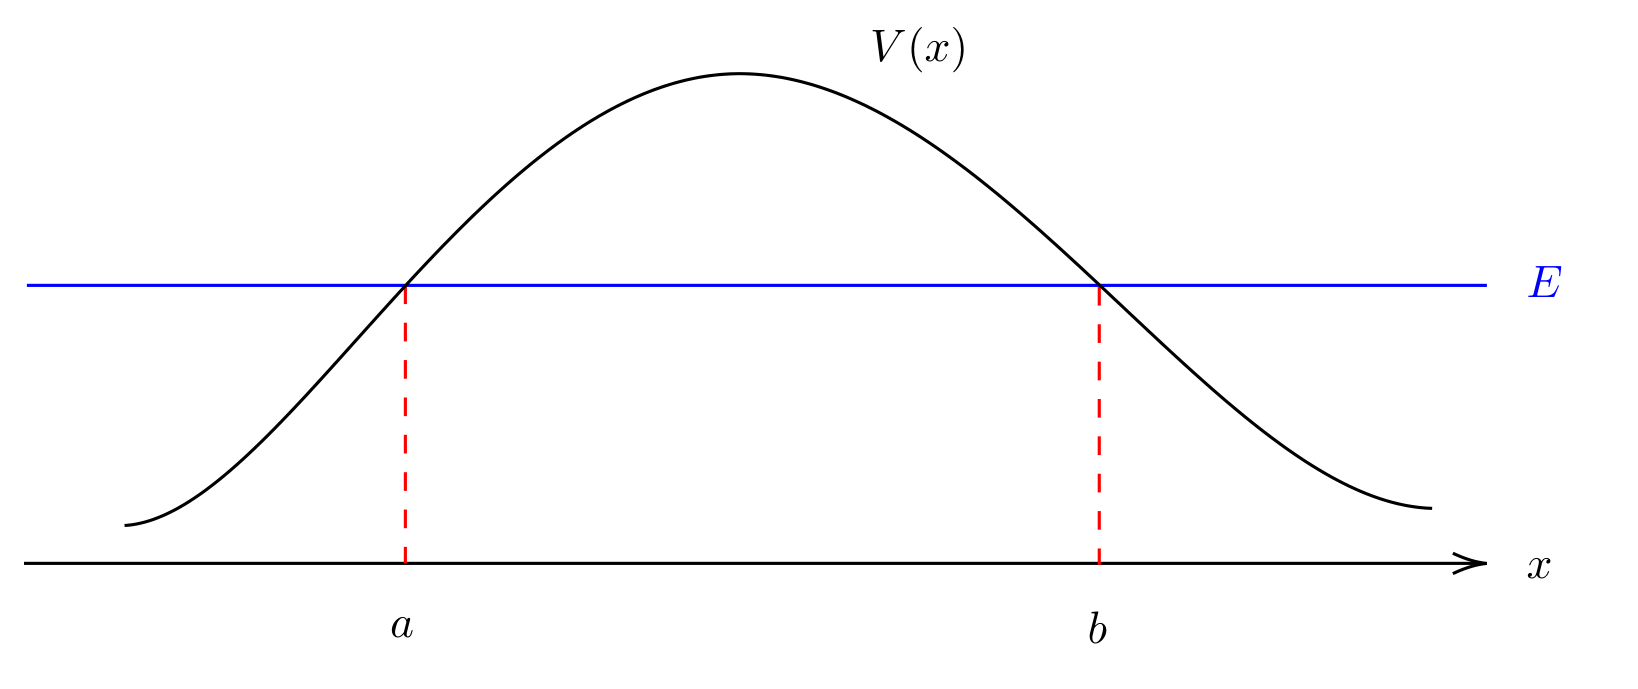
\includegraphics[width=0.68\textwidth]{figures/fig_p133_a.png}
\end{center}
% [图：原书 p.132，图内文字照原样保留]

正如我们在例 2.7.3 中看到的，格林函数的行为为
\[
G(x'',x';E)=\frac{m}{\ii k\hs^2}A\ee^{\ii k(x''-x')},
\qquad x'\to-\infty,\ x''\to+\infty,
\]
其中 $A$ 是透射振幅。

另一方面，我们有半经典渐近结果
\[
G(x'',x';E)\simeq\sum_{(x_{cl},T_s)}\frac{1}{\hs}
\left(\frac{1}{-\dot x_{cl}(0)\dot x_{cl}(T_s)}\right)^{\frac12}
\ee^{\frac{\ii}{\hs}W_{cl}}.
\]
注意在极限区域 $x'\to-\infty$、$x''\to+\infty$，粒子变为自由粒子，速度为
\[
\dot x(0)=\dot x(T_s)=\frac{\hs k}{m},
\]
其中 $k=\frac{\sqrt{2mE}}{\hs}$。

要有一条从 $x'$ 到 $x''$、沿 $t=0$ 到 $t=T$ 的时间路径的经典轨道，就必须经过一段复时间！这是因为 $x'$ 与 $x''$ 都位于经典允许区，而路径必须穿过它们之间的经典禁区。要穿透势垒，时间必须是复的。事实上，
\[
\frac{\rd x}{\rd t}=\sqrt{\frac{2(E-V(x))}{m}},
\]

% [原文 p.133]
因此在区域 $E<V(x)$ 中，$t$ 必须沿虚方向。

该轨道的总旅行时间为
\[
\begin{aligned}
T_s&=\int_0^{T_s}\rd t=\int_{x'}^{x''}\frac{\rd x}{\frac{\rd x}{\rd t}}
=\int_{x'}^{x''}\sqrt{\frac{m}{2(E-V(x))}}\,\rd x\\
&=\int_{x'}^{a}\sqrt{\frac{m}{2(E-V(x))}}\,\rd x
+\int_b^{x''}\sqrt{\frac{m}{2(E-V(x))}}\,\rd x
-\underbrace{\ii\int_a^b\sqrt{\frac{m}{2(V(x)-E)}}\,\rd x}_{\text{复时间的虚贡献}}.
\end{aligned}
\]

对这条复时间中的经典轨道，我们有
\[
\begin{aligned}
W_{cl}&=\int_{x'}^{x''}p\,\rd x
=\int_{x'}^{a}\sqrt{2m(E-V(x))}\,\rd x
+\ii\int_a^b\sqrt{2m(V(x)-E)}\,\rd x\\
&\qquad+\int_b^{x''}\sqrt{2m(E-V(x))}\,\rd x.
\end{aligned}
\]
于是半经典格林函数在极限区域 $x'\to-\infty$、$x''\to+\infty$ 为
\[
G(x'',x';E)\simeq\frac{m}{\ii\hs^2k}
\ee^{\frac{\ii}{\hs}\left(\int_{x'}^{a}+\int_b^{x''}\right)
\sqrt{2m(E-V(x))}\,\rd x}
\ee^{-\frac{1}{\hs}\int_a^b\sqrt{2m(V(x)-E)}\,\rd x}.
\]
与结果
\[
G(x'',x';E)=\frac{m}{\ii k\hs^2}A\ee^{\ii k(x''-x')}
\]
比较，我们推得半经典透射系数
\[
T\simeq|A|^2=\ee^{-\frac{2}{\hs}\int_a^b\sqrt{2m(V(x)-E)}\,\rd x}.
\]
这正是第 1.10.5 节中用 WKB 方法算出的公式。

\subsubsection*{连接公式再探}

下面我们考察 WKB 近似在转折点附近的连接公式，那里势近似为线性势，比如
\[
V(x)=-\lambda x,\qquad\lambda>0.
\]
我们假设能量 $E=0$，于是转折点为 $x=0$。

考虑格林函数 $G(x'',x';E=0)$。让我们固定 $x''>0$，并让 $x'$ 从区域 $x'>0$ 变到区域 $x'<0$。
\[
0<x'<x''\qquad\Longrightarrow\qquad x'<0<x''.
\]
\begin{center}
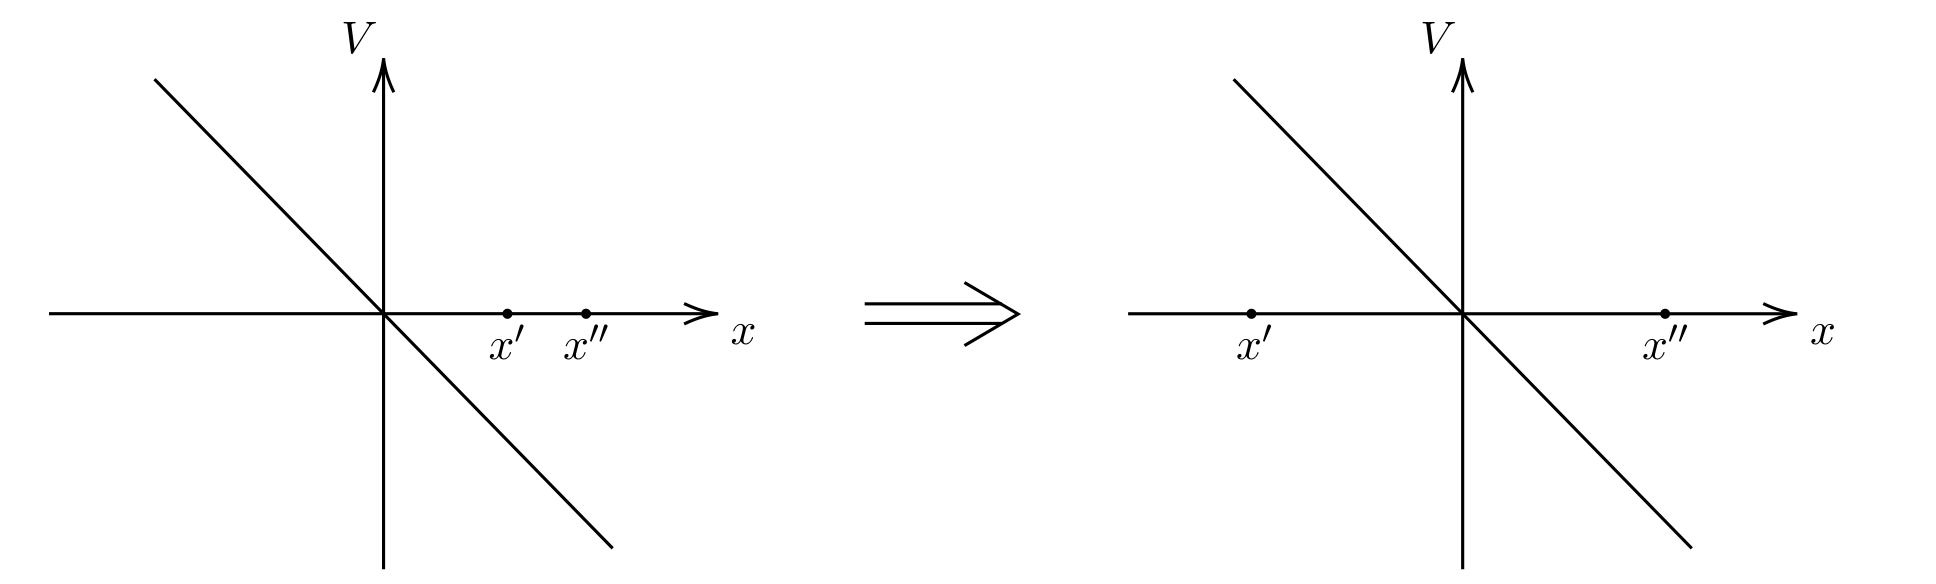
\includegraphics[width=0.75\textwidth]{figures/fig_p134_a.png}
\end{center}
% [图：原书 p.133，图内文字照原样保留]

% [原文 p.134]
我们想沿 $x'$ 的形变追踪半经典近似。然而，若让 $x'$ 沿实轴简单变化，那么当 $x'$ 撞到转折点 $0$ 时很快就会出问题。事实上当 $x'=0$ 时，转折点处的速度为零
\[
\sqrt{\frac{2(E-V)}{m}}=0\qquad\text{在 }x=0\text{ 处}.
\]
于是半经典近似失效，我们失去对渐近信息的追踪。

取而代之，我们可以考虑复平面中的解析延拓，以绕过转折点。例如，我们考察变化
\[
x'=r\ee^{\ii\theta},\qquad r>0
\]
其中 $\theta$ 从 $\theta=0$ 变到 $\theta=\pi$。
\begin{center}
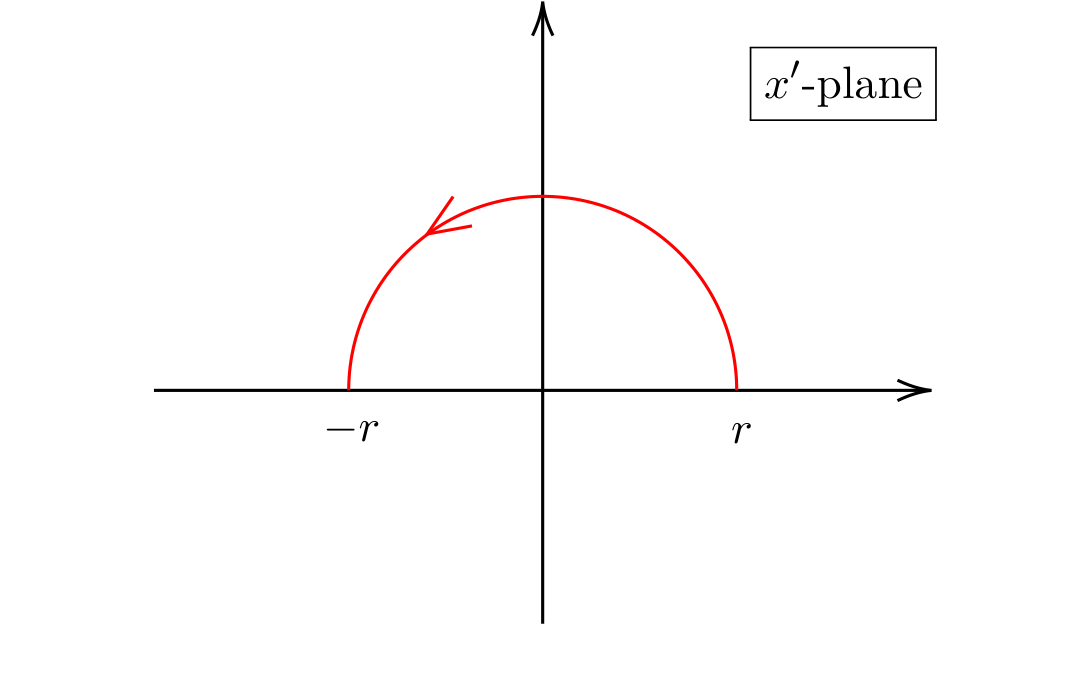
\includegraphics[width=0.55\textwidth]{figures/fig_p135_a.png}
\end{center}
% [图：原书 p.134，图内文字照原样保留]
\nopagebreak[4]
\fignote{图内文字：$x'$-plane（$x'$ 平面）}

正如我们在例 2.7.6 中看到的，$G(x'',x';0)$ 的半经典渐近行为由图中的最速下降曲线贡献
\begin{center}
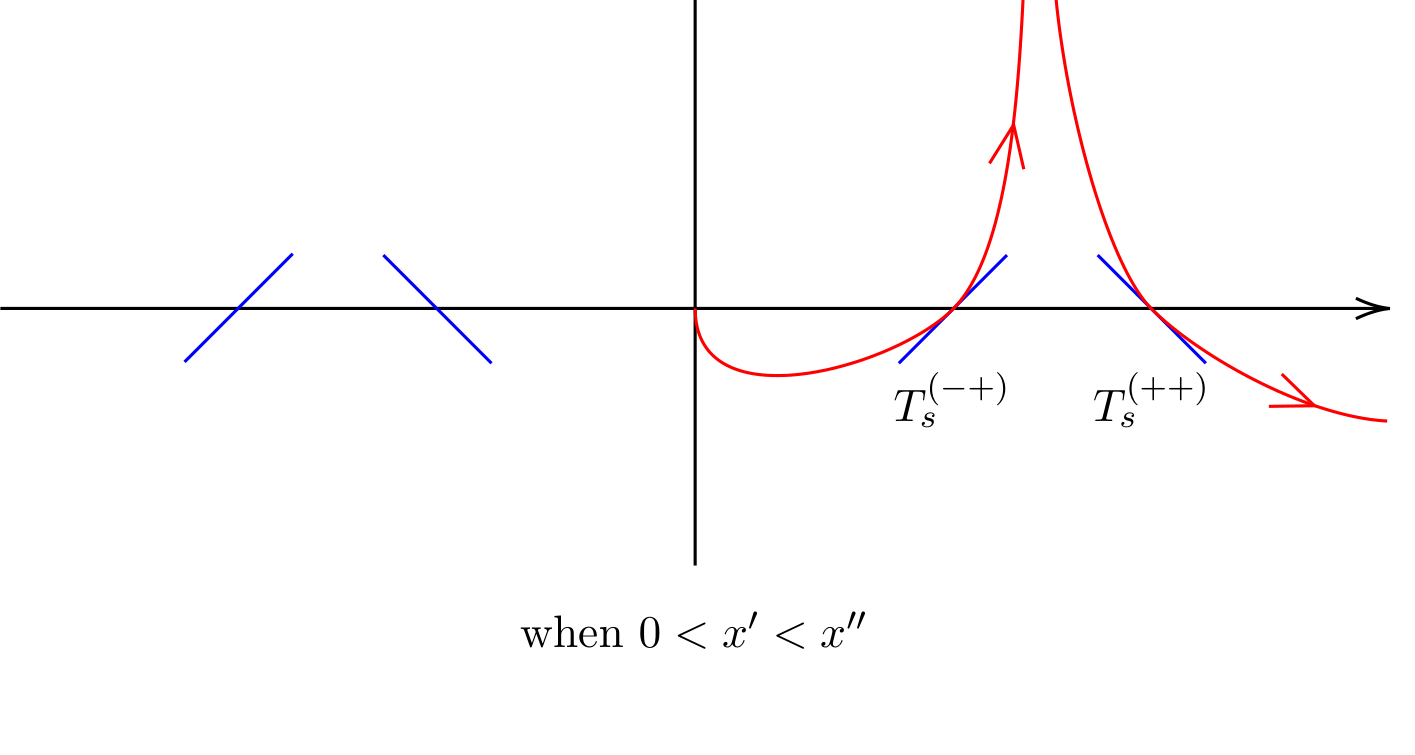
\includegraphics[width=0.68\textwidth]{figures/fig_p135_b.png}
\end{center}
% [图：原书 p.134，图内文字照原样保留]
\nopagebreak[4]
\fignote{图内文字：when $0<x'<x''$（当 $0<x'<x''$ 时）}

% [原文 p.135]
\begin{center}
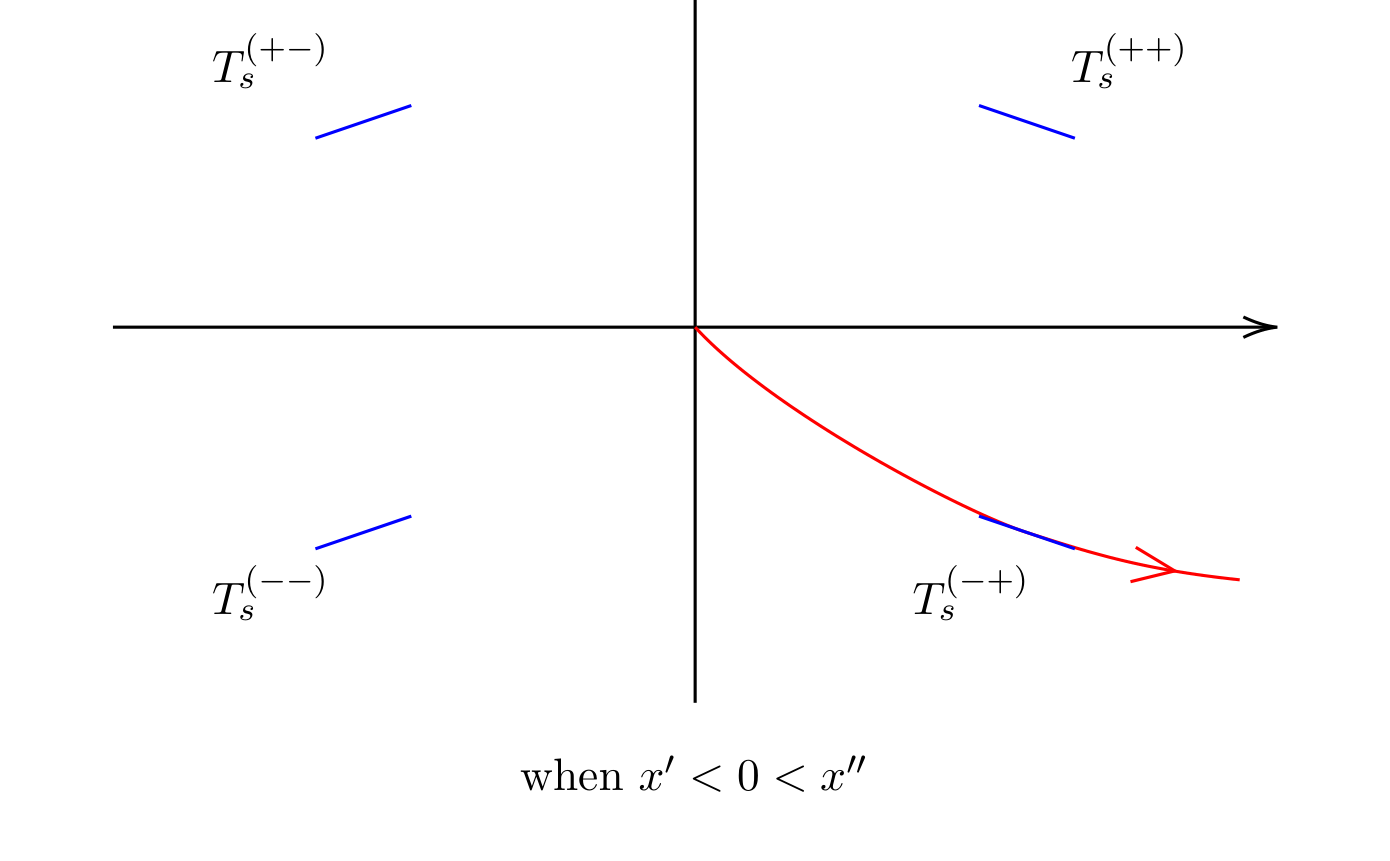
\includegraphics[width=0.66\textwidth]{figures/fig_p136_a.png}
\end{center}
% [图：原书 p.135，图内文字照原样保留]
\nopagebreak[4]
\fignote{图内文字：when $x'<0<x''$（当 $x'<0<x''$ 时）}

让我们分析当 $\theta$ 变化时中间发生了什么。回顾四个鞍点
\[
\begin{aligned}
T_s^{(\pm\pm)}&=\left(\frac{2m}{\lambda}\right)^{\frac12}
\left(\pm\sqrt{x'}\pm\sqrt{x''}\right)\\
&=\left(\frac{2m}{\lambda}\right)^{\frac12}
\left(\pm\ee^{\frac{\ii\theta}{2}}\sqrt r\pm\sqrt{x''}\right),
\qquad 0<r<x''.
\end{aligned}
\]
$S_{cl}$ 在这些鞍点处的值为
\[
S_{cl}\left(T_s^{(\pm\pm)}\right)
=\frac23(2m\lambda)^{\frac12}\left(\pm\sqrt{x'}^3\pm\sqrt{x''}^3\right)
=\frac23(2m\lambda)^{\frac12}\left(\pm\ee^{\frac{3\ii\theta}{2}}\sqrt r^3\pm\sqrt{x''}^3\right).
\]
回顾最速下降曲线满足
\begin{itemize}
\item $\Imag(\ii S_{cl})=\Real(S_{cl})=\text{常数}$；
\item $\Real(\ii S_{cl})=-\Imag(S_{cl})\to-\infty$（沿边界）。
\end{itemize}

在初始阶段
\[
0<x'<x''
\]
有两个贡献鞍点 $T_s^{(-+)}$ 与 $T_s^{(++)}$。考虑
\[
\begin{aligned}
S_{cl}\left(T_s^{(-+)}\right)&=\frac23(2m\lambda)^{\frac12}
\left(-\ee^{\frac{3\ii\theta}{2}}\sqrt r^3+\sqrt{x''}^3\right),\\
S_{cl}\left(T_s^{(++)}\right)&=\frac23(2m\lambda)^{\frac12}
\left(\ee^{\frac{3\ii\theta}{2}}\sqrt r^3+\sqrt{x''}^3\right).
\end{aligned}
\]
当 $\theta$ 变化时，渐近行为的各鞍点贡献可能因斯托克斯现象而跳变，此时某条最速下降曲线可能撞到另一个鞍点。斯托克斯现象发生于
\[
\Real\left(S_{cl}\left(T_s^{(-+)}\right)\right)
=\Real\left(S_{cl}\left(T_s^{(++)}\right)\right),
\]
即当 $\theta=\frac{\pi}{3}$ 时。我们可以画出 $\theta=\frac{\pi}{3}$ 时相应的四个鞍点、鞍点处最速下降的切方向，以及有贡献的最速下降曲线

% [原文 p.136]
\begin{center}
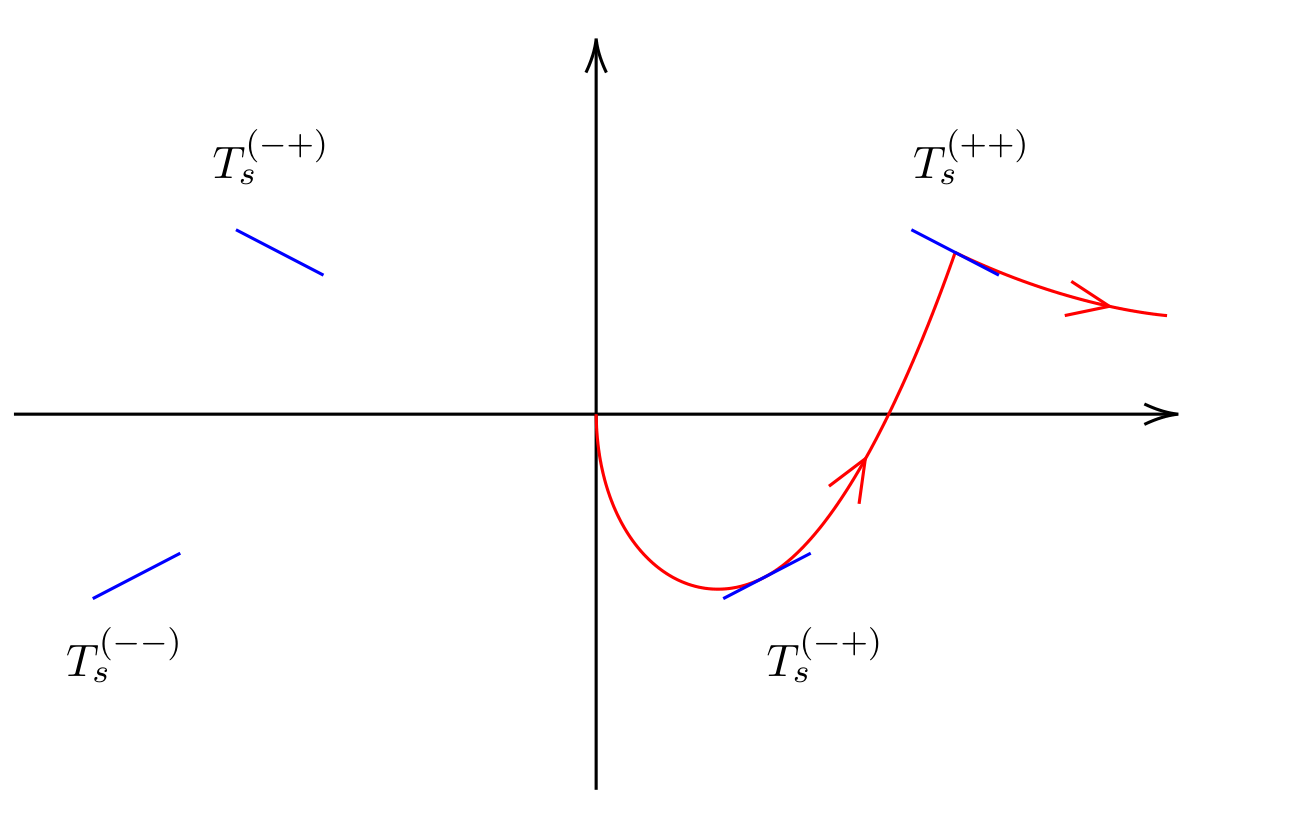
\includegraphics[width=0.66\textwidth]{figures/fig_p137_a.png}
\end{center}
% [图：原书 p.136，图内文字照原样保留]

经过 $\theta=\frac{\pi}{3}$ 之后，只有鞍点 $T_s^{(-+)}$ 对半经典格林函数有贡献。这一过程可以用下图说明
\begin{center}
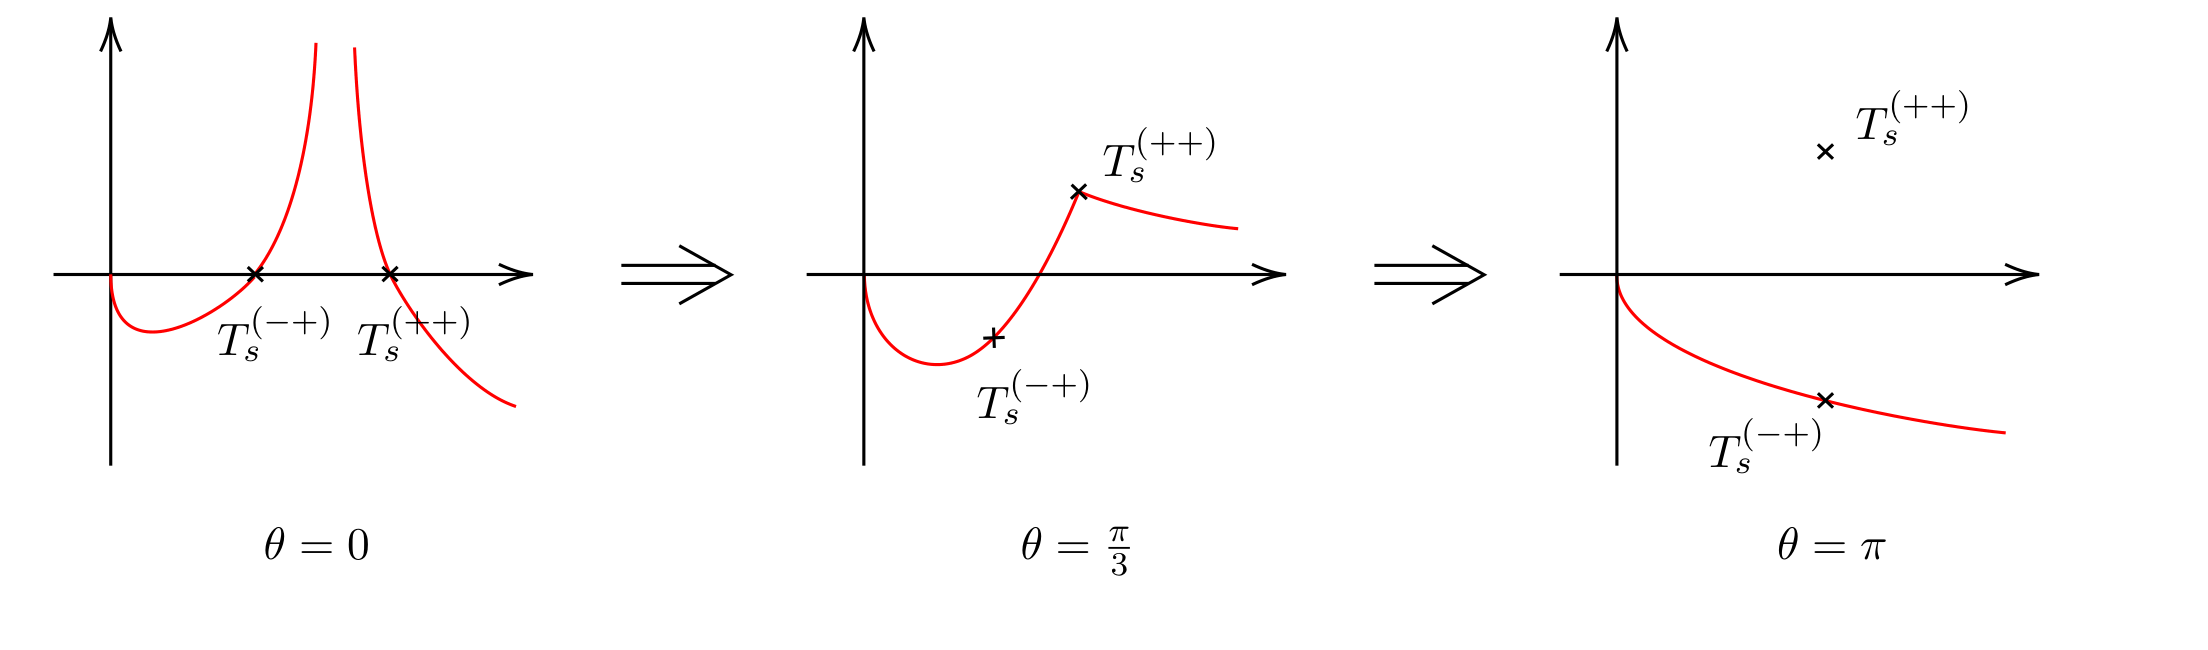
\includegraphics[width=0.75\textwidth]{figures/fig_p137_b.png}
\end{center}
% [图：原书 p.136，图内文字照原样保留]

这一过程解释了连接公式如何起作用。在 $\theta=0$ 时，我们有两个鞍点贡献，来自 $T_s^{(-+)}$ 与 $T_s^{(++)}$，相位因子为
\[
\ee^{\frac{\ii}{\hs}S_{cl}\left(T_s^{(-+)}\right)}
=\ee^{\frac{\ii}{\hs}\frac23(2m\lambda)^{\frac12}
\left(-\sqrt{x'}^3+\sqrt{x''}^3\right)},
\]
\[
\ee^{\frac{\ii}{\hs}S_{cl}\left(T_s^{(++)}\right)}
=\ee^{\frac{\ii}{\hs}\frac23(2m\lambda)^{\frac12}
\left(\sqrt{x'}^3+\sqrt{x''}^3\right)}.
\]
它们对半经典渐近给出同等的主导贡献。

在 $\theta=\pi$ 时，经过 $\theta=\frac{\pi}{3}$ 处的斯托克斯跳跃后，只有 $T_s^{(-+)}$ 对半经典渐近有贡献，相位因子为
\[
\ee^{\frac{\ii}{\hs}S_{cl}\left(T_s^{(-+)}\right)}
=\ee^{\frac{\ii}{\hs}\frac23(2m\lambda)^{\frac12}\sqrt{x''}^3}
\ee^{-\frac{1}{\hs}\frac23(2m\lambda)^{\frac12}\sqrt{-x'}^3}.
\]

类似地，让我们考虑当我们让 $x''$ 变化时格林函数的半经典行为

% [原文 p.137]
\[
x'<x''<0\qquad\Longrightarrow\qquad x'<0<x''.
\]
\begin{center}
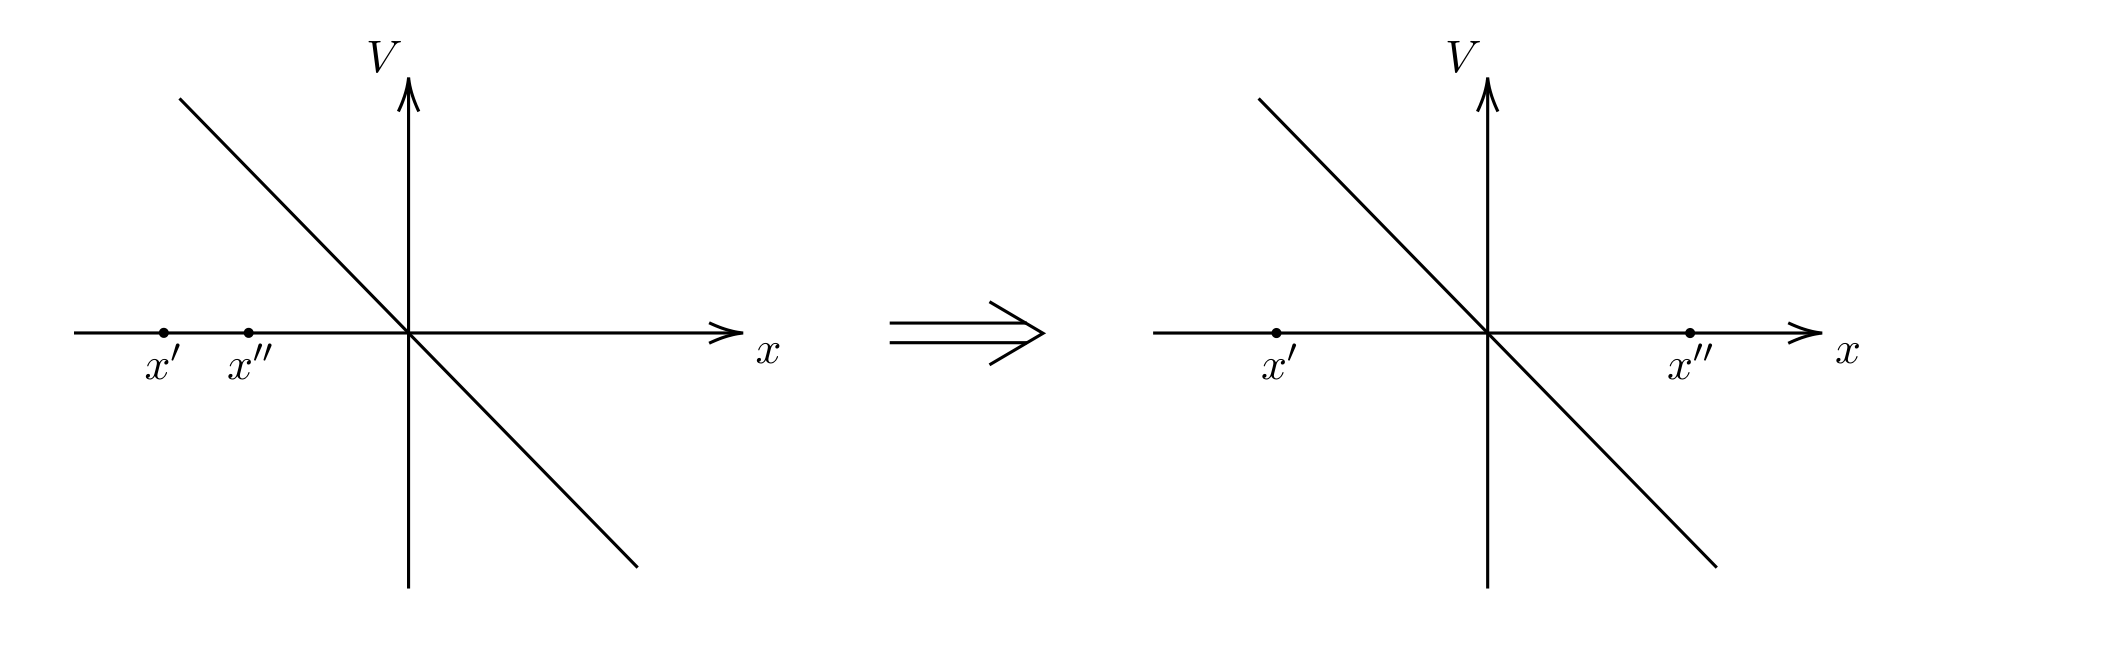
\includegraphics[width=0.86\textwidth]{figures/fig_p137_top.png}
\end{center}
% [图：原书 p.137，图内仅有数学符号标注]

\begin{center}
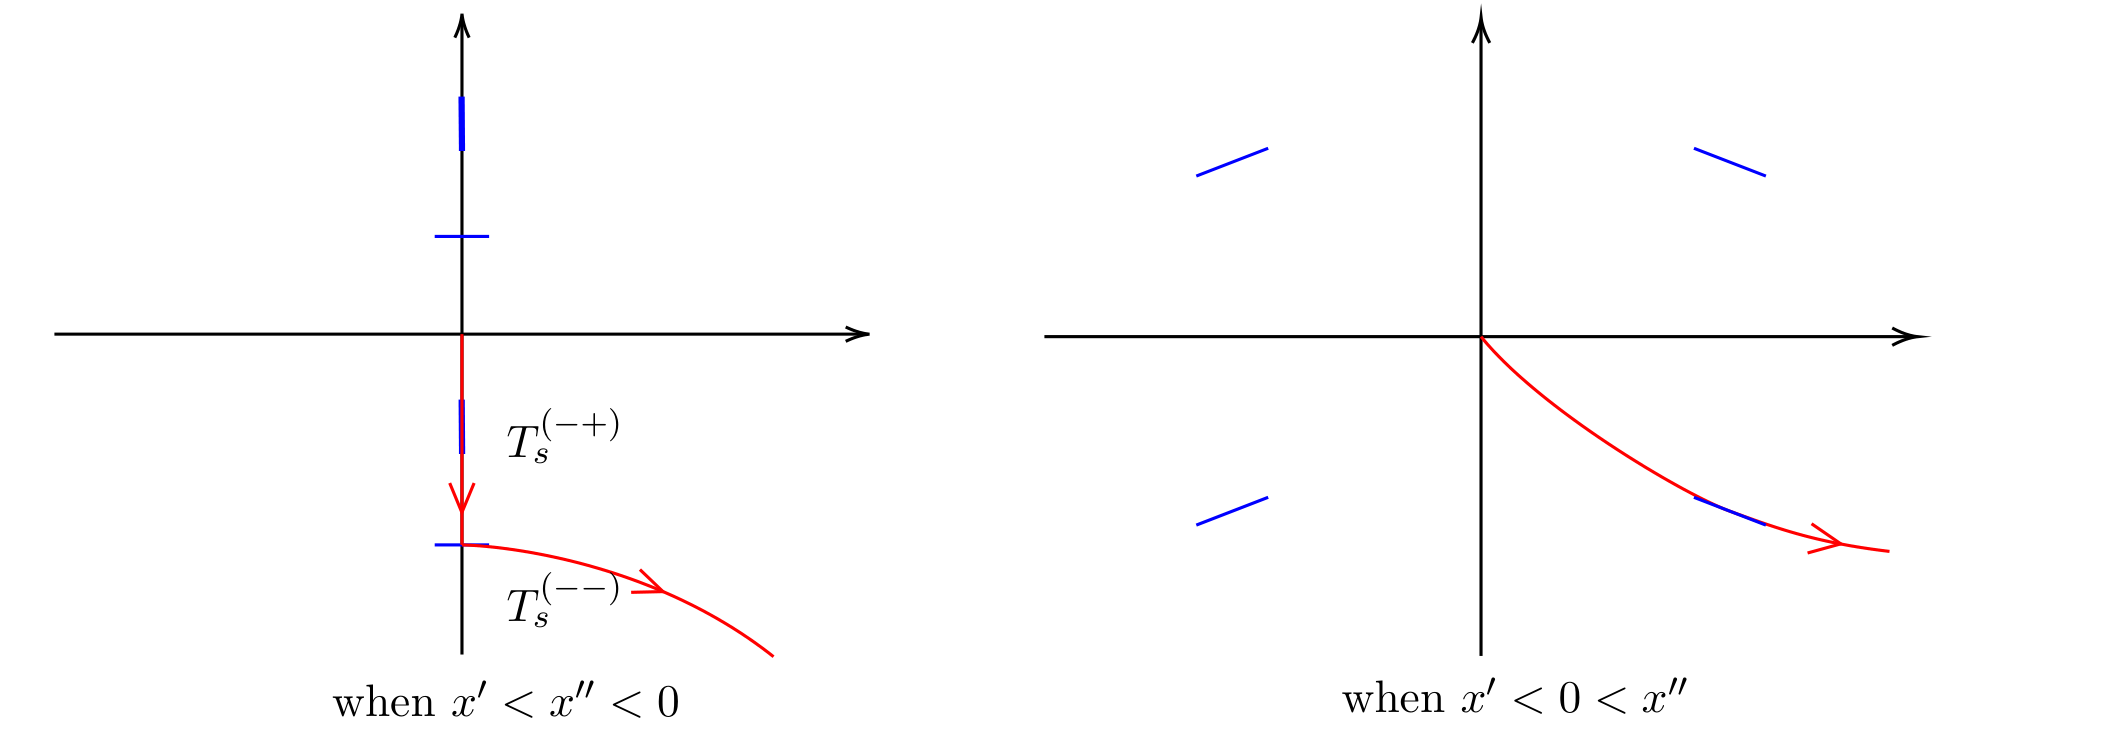
\includegraphics[width=0.86\textwidth]{figures/fig_p137_mid.png}
\end{center}
% [图：原书 p.137，图内文字照原样保留]
\nopagebreak[4]
\fignote{图内文字：when $x'<x''<0$ 与 when $x'<0<x''$（当 $x'<x''<0$ 时与当 $x'<0<x''$ 时）}

当 $x'<x''<0$ 时，我们有两个鞍点贡献，来自 $T_s^{(-+)}$ 与 $T_s^{(--)}$，且
\[
\ee^{\frac{\ii}{\hs}S_{cl}\left(T_s^{(-+)}\right)}
=\ee^{\frac{\ii}{\hs}\frac23(2m\lambda)^{\frac12}
\left(-\sqrt{-x'}^3+\sqrt{-x''}^3\right)},
\]
\[
\ee^{\frac{\ii}{\hs}S_{cl}\left(T_s^{(--)}\right)}
=\ee^{\frac{\ii}{\hs}\frac23(2m\lambda)^{\frac12}
\left(-\sqrt{-x'}^3-\sqrt{-x''}^3\right)}.
\]
来自 $T_s^{(-+)}$ 的鞍点贡献支配来自 $T_s^{(--)}$ 的贡献。

另一个有趣的现象是：从 $T_s^{(--)}$ 出发的最速下降曲线，只有从 $T_s^{(--)}$ 出发的完整最速下降曲线的一半
\begin{center}
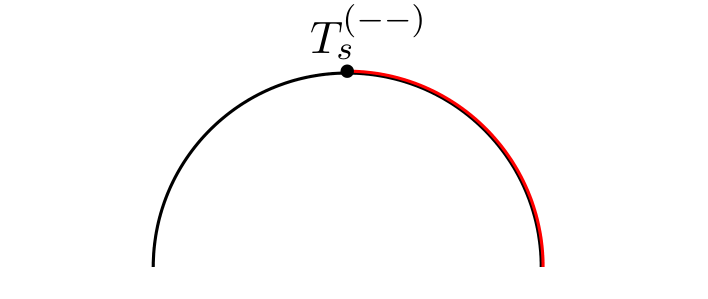
\includegraphics[width=0.30\textwidth]{figures/fig_p137_bot.png}
\end{center}
% [图：原书 p.137，图内文字照原样保留]

当我们计算半经典贡献时，它给出高斯积分通常公式的 $\frac12$。因此我们在这一情形下把鞍点贡献写成
\[
T_s^{(-+)}+\frac12T_s^{(--)}.
\]
当我们让 $x''$ 从区域 $x''<0$ 变到区域 $x''>0$ 时，这两条最速下降曲线将形变为一条最速下降曲线，如图所示。

仔细的计算表明，转折点两侧半经典渐近之间的上述关系，恰好给出 WKB 连接公式（见 [9]）。

\takeaway{本节构造固定能量下的格林函数并作半经典分析：鞍点方程给出经典轨道与旅行时间，分情形讨论 $x'$、$x''$ 在允许区或禁区的位置；转折点附近转为解析延拓，借斯托克斯跳跃导出连接公式，复现 WKB 隧穿系数。}

